\documentclass[twocolumn,superscriptaddress,prd]{revtex4-1} 

\pdfoutput=1 

%\usepackage{hyperref}
\usepackage{verbatim}
%\usepackage[font=normalsize]{caption}
\usepackage{mathtools}
\usepackage{relsize}
\usepackage{natbib}

\usepackage{amsmath}
\usepackage{graphicx}
\usepackage[capposition=bottom]{floatrow}
\usepackage{amssymb}
\usepackage{graphicx}
%\usepackage{caption}
\usepackage{rotating}
\usepackage{afterpage}
\usepackage{float}
\usepackage{geometry}
\usepackage{titlesec}
\usepackage{epstopdf}

\usepackage{latexsym}
\usepackage{graphicx}
\usepackage{color}
\usepackage{array}
\usepackage{multirow}
\usepackage{wasysym}
\usepackage{verbatim}
\usepackage{subfig}


%switch from two to one column



\addtolength{\oddsidemargin}{-.500in}
\addtolength{\evensidemargin}{-.375in}
\addtolength{\textwidth}{1.00in}
%\addtolength{\voffset}{-70pt}
%\addtolength{\textheight} {120pt}
\newcommand{\isot}[2]{$^{#2}$#1 }
\newcommand{\xeiso}{\isot{Xe}{136}}
\newcommand{\thsrc}{\isot{Th}{228}}
\newcommand{\cosrc}{\isot{Co}{60}}
\newcommand{\krsrc}{\isot{Kr}{83m}}
\newcommand{\cssrc}{\isot{Cs}{137}}
\newcommand{\kevee}{keV$_{ee}$ }
\newcommand{\nonubb}  {$0\nu \beta \beta$}
\newcommand{\gone}{$0.116 \pm 0.003$}
\newcommand{\gtwo}{$11.41 \pm 0.52$}
\newcommand{\fixit}[1]{{\color{red}#1}} 

\renewcommand\thesection{\Roman{section}.}
\renewcommand\thesubsection{\arabic{subsection}.}
\renewcommand\thesubsubsection{\alph{subsubsection}.}
\titleformat{\section}[block]{\bfseries\filcenter}{\thesection}{1em}{}
\titleformat{\subsection}[block]{\bfseries\filcenter}{\thesubsection}{1em}{}
\titleformat{\subsubsection}{\bfseries\filcenter}{\thesubsubsection}{1em}{}

\usepackage{titlesec}

%\titleformat{\section}{\bfseries\filcenter}{\thesubsection}{1em}{}
%\titleformat{\subsection}{\bfseries\filcenter}{\thesubsection}{1em}{}
%\titleformat*{\paragraph}{\large\bfseries}
%\titleformat*{\subparagraph}{\large\bfseries}

\begin{document}

\title{Run04 corrections - Knoche Draft / December 2016 plus figures approved April 2016 / Prior to July 2017 revision of the text}


\author{D.S.~Akerib} %% Joined 4/2008
\affiliation{Case Western Reserve University, Department of Physics, 10900 Euclid Ave, Cleveland, OH 44106, USA}
\affiliation{SLAC National Accelerator Laboratory, 2575 Sand Hill Road, Menlo Park, CA 94205, USA}
\affiliation{Kavli Institute for Particle Astrophysics and Cosmology, Stanford University, 452 Lomita Mall, Stanford, CA 94309, USA}

\author{H.M.~Ara\'{u}jo} %% Joined 4/2012, Author on 4/2013
\affiliation{Imperial College London, High Energy Physics, Blackett Laboratory, London SW7 2BZ, United Kingdom}

\author{X.~Bai} %% Joined 7/2009
\affiliation{South Dakota School of Mines and Technology, 501 East St Joseph St., Rapid City, SD 57701, USA}

\author{A.J.~Bailey} %% Joined 1/2013, Author on 1/2014
\affiliation{Imperial College London, High Energy Physics, Blackett Laboratory, London SW7 2BZ, United Kingdom}

\author{J.~Balajthy} %% Joined 7/2012, Author on 7/2013
\affiliation{University of Maryland, Department of Physics, College Park, MD 20742, USA}

%\author{S.~Bedikian} %% Left 2/2010, Author until 2/2012
%\affiliation{Yale University, Department of Physics, 217 Prospect St., New Haven, CT 06511, USA}

\author{P.~Beltrame} %% Joined 10/2013, Author on 10/2014.
\affiliation{SUPA, School of Physics and Astronomy, University of Edinburgh, Edinburgh EH9 3FD, United Kingdom}

\author{E.P.~Bernard} %% Joined 1/2010, Author on 1/2011
\affiliation{Yale University, Department of Physics, 217 Prospect St., New Haven, CT 06511, USA}

\author{A.~Bernstein} %% From the start
\affiliation{Lawrence Livermore National Laboratory, 7000 East Ave., Livermore, CA 94551, USA}

\author{T.P.~Biesiadzinski} %% Joined 10/2013, Author on 10/2014
\affiliation{Case Western Reserve University, Department of Physics, 10900 Euclid Ave, Cleveland, OH 44106, USA}
\affiliation{SLAC National Accelerator Laboratory, 2575 Sand Hill Road, Menlo Park, CA 94205, USA}
\affiliation{Kavli Institute for Particle Astrophysics and Cosmology, Stanford University, 452 Lomita Mall, Stanford, CA 94309, USA}

%\author{A.~Bolozdynya} %% From the start, Left Case 7/09, Author until 7/11
%\affiliation{Case Western Reserve University, Department of Physics, 10900 Euclid Ave, Cleveland, OH 44106, USA}

\author{E.M.~Boulton} %% Joined 3/2013, Author on 3/2014
\affiliation{Yale University, Department of Physics, 217 Prospect St., New Haven, CT 06511, USA}

\author{A.~Bradley} %% From start, Left 12/2013, Author until 12/2015
\affiliation{Case Western Reserve University, Department of Physics, 10900 Euclid Ave, Cleveland, OH 44106, USA}

\author{R.~Bramante} %% Joined 3/2014, Author on 3/2015
\affiliation{Case Western Reserve University, Department of Physics, 10900 Euclid Ave, Cleveland, OH 44106, USA}
\affiliation{SLAC National Accelerator Laboratory, 2575 Sand Hill Road, Menlo Park, CA 94205, USA}
\affiliation{Kavli Institute for Particle Astrophysics and Cosmology, Stanford University, 452 Lomita Mall, Stanford, CA 94309, USA}

%\author{D.~Byram} %% Joined 10/2010, Left 3/2013, Author until 3/2015
%\affiliation{University of South Dakota, Department of Physics, 414E Clark St., Vermillion, SD 57069, USA}

\author{S.B.~Cahn} %% Joined 2/2009, Left 12/2012, Worked on Kr source in 2015, Author until 12/2017
\affiliation{Yale University, Department of Physics, 217 Prospect St., New Haven, CT 06511, USA}

\author{M.C.~Carmona-Benitez} %% Joined 10/2009, Moved from Case to UCSB 7/31/2013
\affiliation{University of California Santa Barbara, Department of Physics, Santa Barbara, CA 93106, USA}

%\author{D. Carr} %% From start, Left on ??
%\affiliation{Lawrence Livermore National Laboratory, 7000 East Ave., Livermore, CA 94551, USA}

\author{C.~Chan} %% Joined 8/2012, Author on 8/2013
\affiliation{Brown University, Department of Physics, 182 Hope St., Providence, RI 02912, USA}

\author{J.J.~Chapman} %% Joined 6/2007, Author on 6/2008, Left on 1/2014, Author until 1/2016
\affiliation{Brown University, Department of Physics, 182 Hope St., Providence, RI 02912, USA}

\author{A.A.~Chiller} %% Joined 11/2011, Author on 11/2012
\affiliation{University of South Dakota, Department of Physics, 414E Clark St., Vermillion, SD 57069, USA}

\author{C.~Chiller} %% Joined 11/2011, Author on 11/2012
\affiliation{University of South Dakota, Department of Physics, 414E Clark St., Vermillion, SD 57069, USA}

%\author{K.~Clark} %% Joined 6/2008, Left 6/2010, Author until 6/2012
%\affiliation{Case Western Reserve University, Department of Physics, 10900 Euclid Ave, Cleveland, OH 44106, USA}

%\author{T.~Classen} %% Joined 10/2007, Left 11/2009, Author until 11/2011
%  address={University of California Davis, Department of Physics, One Shields Ave., Davis, CA 95616, USA}

%\author{T.~Coffey} %% Joined 8/2010, Left 8/2012, Author until 8/2014
%\affiliation{Case Western Reserve University, Department of Physics, 10900 Euclid Ave, Cleveland, OH 44106, USA}

\author{A.~Currie} %% Joined 4/2012, Author on 4/2013
\affiliation{Imperial College London, High Energy Physics, Blackett Laboratory, London SW7 2BZ, United Kingdom}

%\author{A.~Curioni} %% Left 6/2009, Author until 6/2011
%\affiliation{Yale University, Department of Physics, 217 Prospect St., New Haven, CT 06511, USA}

\author{J.E.~Cutter}  %% Joined 8/2013, Author on 8/2014
\affiliation{University of California Davis, Department of Physics, One Shields Ave., Davis, CA 95616, USA}

%\author{E.~Dahl} %% From start; Left ???
%\affiliation{Case Western Reserve University, Department of Physics, 10900 Euclid Ave, Cleveland, OH 44106, USA}

\author{T.J.R.~Davison} %% Joined 2/2014, Author on 2/2015.
\affiliation{SUPA, School of Physics and Astronomy, University of Edinburgh, Edinburgh EH9 3FD, United Kingdom}

%\author{S.~Dazeley} %% From start, Left ?
%\affiliation{Lawrence Livermore National Laboratory, 7000 East Ave., Livermore, CA 94551, USA}

\author{L.~de\,Viveiros} %% From the start (at Brown), moved to Coimbra, Left 1/1/2014, Author until 1/1/2016. 
\affiliation{LIP-Coimbra, Department of Physics, University of Coimbra, Rua Larga, 3004-516 Coimbra, Portugal}

\author{A.~Dobi} %% Joined 7/2011, Author on 7/2012
\affiliation{Lawrence Berkeley National Laboratory, 1 Cyclotron Rd., Berkeley, CA 94720, USA}

\author{J.E.Y.~Dobson} %% Joined 09/2012, Author on 09/2013, Left 7/2015, Author until 7/2017
\affiliation{Department of Physics and Astronomy, University College London, Gower Street, London WC1E 6BT, United Kingdom}

%\author{E.~Dragowsky} %% Joined 01/09, Left 10/11, Author until 10/13
%\affiliation{Case Western Reserve University, Department of Physics, 10900 Euclid Ave, Cleveland, OH 44106, USA}

\author{E.~Druszkiewicz} %% From the start
\affiliation{University of Rochester, Department of Physics and Astronomy, Rochester, NY 14627, USA}

\author{B.N.~Edwards} %% Joined 3/2011, Author on 3/2012.
\affiliation{Yale University, Department of Physics, 217 Prospect St., New Haven, CT 06511, USA}

\author{C.H.~Faham} %% Joined June 2007, Moved from Brown to Berkeley 9/1/2013, Left 6/2015, Author until 6/2017
\affiliation{Lawrence Berkeley National Laboratory, 1 Cyclotron Rd., Berkeley, CA 94720, USA}

\author{S.~Fiorucci} %% From start
\affiliation{Brown University, Department of Physics, 182 Hope St., Providence, RI 02912, USA}

%\author{C.~Flores} %% Joined 10/2012, Left 10/2012
%\affiliation{University of California Davis, Department of Physics, One Shields Ave., Davis, CA 95616, USA}

\author{R.J.~Gaitskell} %% From start
\affiliation{Brown University, Department of Physics, 182 Hope St., Providence, RI 02912, USA}

\author{V.M.~Gehman} %% Joined 5/2012, Author on 5/2013, Left 6/2015, Author until 6/2017
\affiliation{Lawrence Berkeley National Laboratory, 1 Cyclotron Rd., Berkeley, CA 94720, USA}

\author{C.~Ghag} %% Joined 6/2012, Author on 6/2013
\affiliation{Department of Physics and Astronomy, University College London, Gower Street, London WC1E 6BT, United Kingdom}

\author{K.R.~Gibson} %% Joined 10/2009, Left 9/2014, Author until 9/2016
\affiliation{Case Western Reserve University, Department of Physics, 10900 Euclid Ave, Cleveland, OH 44106, USA}

\author{M.G.D.~Gilchriese} %% Joined 10/2010, Author on 10/2011
\affiliation{Lawrence Berkeley National Laboratory, 1 Cyclotron Rd., Berkeley, CA 94720, USA}

\author{C.R.~Hall} %% Joined 3/2008, Author on 3/2009
\affiliation{University of Maryland, Department of Physics, College Park, MD 20742, USA}

\author{M.~Hanhardt} %% Joined 7/2009, Left 8/2011, Rejoined 7/2013, Author on 7/2014
\affiliation{South Dakota School of Mines and Technology, 501 East St Joseph St., Rapid City, SD 57701, USA}
\affiliation{South Dakota Science and Technology Authority, Sanford Underground Research Facility, Lead, SD 57754, USA}

\author{S.J.~Haselschwardt}  %% Joined 6/2013, Author on 6/2014
\affiliation{University of California Santa Barbara, Department of Physics, Santa Barbara, CA 93106, USA}

\author{S.A.~Hertel} %% Joined 9/2012, Author on 9/2013
\affiliation{University of California Berkeley, Department of Physics, Berkeley, CA 94720, USA}
\affiliation{Yale University, Department of Physics, 217 Prospect St., New Haven, CT 06511, USA}

\author{D.P.~Hogan} %% Joined 2/2014, Author on 2/2015
\affiliation{University of California Berkeley, Department of Physics, Berkeley, CA 94720, USA}

%\author{B.~Holbrook} %% Engineer, Joined 12/2007
%  address={University of California Davis, Department of Physics, One Shields Ave., Davis, CA 95616, USA}

\author{M.~Horn} %% Joined 4/2012, Author on 4/2013.
\affiliation{University of California Berkeley, Department of Physics, Berkeley, CA 94720, USA}
\affiliation{Yale University, Department of Physics, 217 Prospect St., New Haven, CT 06511, USA}

\author{D.Q.~Huang} %% Joined 7/2012, Author on 7/2013
\affiliation{Brown University, Department of Physics, 182 Hope St., Providence, RI 02912, USA}

\author{C.M.~Ignarra} %% Joined 10/2014, Author on 10/2015
\affiliation{SLAC National Accelerator Laboratory, 2575 Sand Hill Road, Menlo Park, CA 94205, USA}
\affiliation{Kavli Institute for Particle Astrophysics and Cosmology, Stanford University, 452 Lomita Mall, Stanford, CA 94309, USA}

\author{M.~Ihm} %% Joined 10/2009, Author on 10/2010
\affiliation{University of California Berkeley, Department of Physics, Berkeley, CA 94720, USA}

%\author{T. Ivancic} %% Joined 1/2012, Left 6/2012, Never an author.
%  address={Case Western Reserve University, Department of Physics, 10900 Euclid Ave, Cleveland, OH 44106, USA}

\author{R.G.~Jacobsen} %% Joined 12/2009, Author on 12/2010
\affiliation{University of California Berkeley, Department of Physics, Berkeley, CA 94720, USA}

\author{W.~Ji} %% Joined 3/2014, Author on 3/2015
\affiliation{Case Western Reserve University, Department of Physics, 10900 Euclid Ave, Cleveland, OH 44106, USA}
\affiliation{SLAC National Accelerator Laboratory, 2575 Sand Hill Road, Menlo Park, CA 94205, USA}
\affiliation{Kavli Institute for Particle Astrophysics and Cosmology, Stanford University, 452 Lomita Mall, Stanford, CA 94309, USA}

%\author{K.~Kamdin %% Joined 3/2015, Author on 3/2016
%\affiliation{University of California Berkeley, Department of Physics, Berkeley, CA 94720, USA}

%\author{L.~Kastens} %% Joined 6/2007, Left 7/2011, Author until 7/2013
%\affiliation{Yale University, Department of Physics, 217 Prospect St., New Haven, CT 06511, USA}

\author{K.~Kazkaz} %% From start
\affiliation{Lawrence Livermore National Laboratory, 7000 East Ave., Livermore, CA 94551, USA}

\author{D.~Khaitan} %% Joined 6/2014, Author on 6/2015
\affiliation{University of Rochester, Department of Physics and Astronomy, Rochester, NY 14627, USA}

\author{R.~Knoche} %% Joined 7/2011, Author on 7/2012
\affiliation{University of Maryland, Department of Physics, College Park, MD 20742, USA}

%\author{S.~Kyre} %% Engineer, Joined 6/2010
%\affiliation{University of California Santa Barbara, Department of Physics, Santa Barbara, CA 93106, USA}

%\author{R.~Lander} %% Joined 3/2008, Decided not to be a LUX author.
%\affiliation{University of California Davis, Department of Physics, One Shields Ave., Davis, CA 95616, USA}

\author{N.A.~Larsen} %% Joined 6/2010, Author on 6/2011
\affiliation{Yale University, Department of Physics, 217 Prospect St., New Haven, CT 06511, USA}

\author{C.~Lee} %% Joined 8/2009
\affiliation{Case Western Reserve University, Department of Physics, 10900 Euclid Ave, Cleveland, OH 44106, USA}
\affiliation{SLAC National Accelerator Laboratory, 2575 Sand Hill Road, Menlo Park, CA 94205, USA}
\affiliation{Kavli Institute for Particle Astrophysics and Cosmology, Stanford University, 452 Lomita Mall, Stanford, CA 94309, USA}

\author{B.G.~Lenardo} %% Joined 7/2013, Author on 7/2014
\affiliation{University of California Davis, Department of Physics, One Shields Ave., Davis, CA 95616, USA}
\affiliation{Lawrence Livermore National Laboratory, 7000 East Ave., Livermore, CA 94551, USA}

%\author{D.S.~Leonard} %% Joined 11/2008, Left 2/2010, Author until 2/2012.
%\affiliation{University of Maryland, Department of Physics, College Park, MD 20742, USA}

\author{K.T.~Lesko} %% Joined 3/2007, Left ?, Rejoined 4/2013, Author on 4/2014
\affiliation{Lawrence Berkeley National Laboratory, 1 Cyclotron Rd., Berkeley, CA 94720, USA}

\author{A.~Lindote} %% Joined 12/2010, Author on 12/2011.
\affiliation{LIP-Coimbra, Department of Physics, University of Coimbra, Rua Larga, 3004-516 Coimbra, Portugal}

\author{M.I.~Lopes} %% Joined 12/2010, Author on 12/2011.
\affiliation{LIP-Coimbra, Department of Physics, University of Coimbra, Rua Larga, 3004-516 Coimbra, Portugal}

%\author{R. Lorek} %% Joined 6/2012, Focussed on R&D for LZ, Will not be an author.
%  address={Case Western Reserve University, Department of Physics, 10900 Euclid Ave, Cleveland, OH 44106, USA}

%\author{A.~Lyashenko} %% Joined 7/2009, Left 8/2011, Author until 8/2013
%\affiliation{Yale University, Department of Physics, 217 Prospect St., New Haven, CT 06511, USA}

\author{D.C.~Malling} %% Joined 8/2007, Author on 8/2008, Left on 12/2013, Author until 12/2015 
\affiliation{Brown University, Department of Physics, 182 Hope St., Providence, RI 02912, USA}

\author{A.G.~Manalaysay} %% Joined 10/2013, Author on 10/2014
\affiliation{University of California Davis, Department of Physics, One Shields Ave., Davis, CA 95616, USA}

\author{R.L.~Mannino} %% Joined 6/2009, Author on 6/2010
\affiliation{Texas A \& M University, Department of Physics, College Station, TX 77843, USA}

\author{M.F.~Marzioni} %% Joined 9/2014, Author on 9/2015
\affiliation{SUPA, School of Physics and Astronomy, University of Edinburgh, Edinburgh EH9 3FD, United Kingdom}

\author{D.N.~McKinsey} %% Joined 6/2007, Author on 6/2008
\affiliation{University of California Berkeley, Department of Physics, Berkeley, CA 94720, USA}
\affiliation{Yale University, Department of Physics, 217 Prospect St., New Haven, CT 06511, USA}

\author{D.-M.~Mei} %% Joined 7/2008
\affiliation{University of South Dakota, Department of Physics, 414E Clark St., Vermillion, SD 57069, USA}

\author{J.~Mock} %% Joined 8/2007
\affiliation{University at Albany, State University of New York, Department of Physics, 1400 Washington Ave., Albany, NY 12222, USA}

\author{M.~Moongweluwan} %% Joined 6/2011, Author on 6/2012.
\affiliation{University of Rochester, Department of Physics and Astronomy, Rochester, NY 14627, USA}

\author{J.A.~Morad} %% Joined 7/2012, Author on 7/2013
\affiliation{University of California Davis, Department of Physics, One Shields Ave., Davis, CA 95616, USA}

%\author{M.~Morii} %% Joined June 09, Left May 2011, Author until May 2013
%\affiliation{Harvard University, Department of Physics, 17 Oxford St., Cambridge MA 02138, USA}

\author{A.St.J.~Murphy} %% Joined 06/2012, Author on 06/2013.
\affiliation{SUPA, School of Physics and Astronomy, University of Edinburgh, Edinburgh EH9 3FD, United Kingdom}

\author{C.~Nehrkorn} %% Joined 5/2012, Author on 5/2013
\affiliation{University of California Santa Barbara, Department of Physics, Santa Barbara, CA 93106, USA}

\author{H.N.~Nelson} %% Joined 11/2008
\affiliation{University of California Santa Barbara, Department of Physics, Santa Barbara, CA 93106, USA}

\author{F.~Neves} %% Joined 12/2010, Author on 12/2011.
\affiliation{LIP-Coimbra, Department of Physics, University of Coimbra, Rua Larga, 3004-516 Coimbra, Portugal}

%\author{J.A.~Nikkel} %% Joined 4/2008, Left 12/2011, Author until 12/2013
%\affiliation{Yale University, Department of Physics, 217 Prospect St., New Haven, CT 06511, USA}

\author{K.~O'Sullivan} %% Joined 9/2012, Author on 9/2013
\affiliation{University of California Berkeley, Department of Physics, Berkeley, CA 94720, USA}
\affiliation{Lawrence Berkeley National Laboratory, 1 Cyclotron Rd., Berkeley, CA 94720, USA}
\affiliation{Yale University, Department of Physics, 217 Prospect St., New Haven, CT 06511, USA}

\author{K.C.~Oliver-Mallory} %% Joined 5/2014, Author on 5/2015
\affiliation{University of California Berkeley, Department of Physics, Berkeley, CA 94720, USA}

\author{R.A.~Ott} %% Joined 3/2012, Author on 3/2013, Left on 3/2014, Author until 3/2016
\affiliation{University of California Davis, Department of Physics, One Shields Ave., Davis, CA 95616, USA}

\author{K.J.~Palladino} %% Joined 10/2013, Author on 10/2014
\affiliation{SLAC National Accelerator Laboratory, 2575 Sand Hill Road, Menlo Park, CA 94205, USA}
\affiliation{Kavli Institute for Particle Astrophysics and Cosmology, Stanford University, 452 Lomita Mall, Stanford, CA 94309, USA}

\author{M.~Pangilinan} %% Joined 2/2010, Left  4/2014, Author until 4/2016
\affiliation{Brown University, Department of Physics, 182 Hope St., Providence, RI 02912, USA}

%\author{P.D.~Parker} %% Joined 9/2010, Active on 12/2011, Left on 6/2013, Author until 6/2015
%\affiliation{Yale University, Department of Physics, 217 Prospect St., New Haven, CT 06511, USA}

\author{E.K.~Pease} %% Joined 12/2011, Author on 12/2012.
\affiliation{Yale University, Department of Physics, 217 Prospect St., New Haven, CT 06511, USA}

%\author{K.~Pech} %% Joined 6/2011, Author on 6/2012, Left 9/2013, Author until 9/2015
%\affiliation{Case Western Reserve University, Department of Physics, 10900 Euclid Ave, Cleveland, OH 44106, USA}

\author{P.~Phelps} %% Joined 6/2008, Left 7/2014, Author until 7/2016
\affiliation{Case Western Reserve University, Department of Physics, 10900 Euclid Ave, Cleveland, OH 44106, USA}

%\author{J.~Pinto~da~Cunha} %% Joined 12/2010, will not be an author until further notice.
%\affiliation{LIP-Coimbra, Department of Physics, University of Coimbra, Rua Larga, 3004-516 Coimbra, Portugal}

\author{L.~Reichhart} %% Joined 6/2012, Author on 6/2013, Left on 5/2015, Author until 5/2017
\affiliation{Department of Physics and Astronomy, University College London, Gower Street, London WC1E 6BT, United Kingdom}

\author{C.~Rhyne} %% Joined 6/2014, Author on 6/2015
\affiliation{Brown University, Department of Physics, 182 Hope St., Providence, RI 02912, USA}

\author{S.~Shaw} %% Joined 2/2014, Author on 2/2015
\affiliation{Department of Physics and Astronomy, University College London, Gower Street, London WC1E 6BT, United Kingdom}

\author{T.A.~Shutt} %% From start
\affiliation{Case Western Reserve University, Department of Physics, 10900 Euclid Ave, Cleveland, OH 44106, USA}
\affiliation{SLAC National Accelerator Laboratory, 2575 Sand Hill Road, Menlo Park, CA 94205, USA}
\affiliation{Kavli Institute for Particle Astrophysics and Cosmology, Stanford University, 452 Lomita Mall, Stanford, CA 94309, USA}

\author{C.~Silva} %% Joined 12/2010, Author on 12/2011.
\affiliation{LIP-Coimbra, Department of Physics, University of Coimbra, Rua Larga, 3004-516 Coimbra, Portugal}

%\author{W.~Skulski} %% From start, Author on trigger-related publications.
%\affiliation{University of Rochester, Department of Physics and Astronomy, Rochester, NY 14627, USA}

\author{V.N.~Solovov} %% Joined 12/2010, Author on 12/2011.
\affiliation{LIP-Coimbra, Department of Physics, University of Coimbra, Rua Larga, 3004-516 Coimbra, Portugal}

\author{P.~Sorensen} %% From start
\affiliation{Lawrence Berkeley National Laboratory, 1 Cyclotron Rd., Berkeley, CA 94720, USA}

%\author{J. Spaans} %% Joined 2/2009, Left 5/2010, Author until 5/2012
%\affiliation{University of South Dakota, Department of Physics, 414E Clark St., Vermillion, SD 57069, USA}

\author{S.~Stephenson}  %% Joined 8/2014, Author on 8/2015
\affiliation{University of California Davis, Department of Physics, One Shields Ave., Davis, CA 95616, USA}

%\author{T. Stiegler} %% Joined 10/2007, Left on 12/2011, Not authorship
%\affiliation{Texas A \& M University, Department of Physics, College Station, TX 77843, USA}

\author{T.J.~Sumner} %% Joined 4/2012, Author on 4/2013
\affiliation{Imperial College London, High Energy Physics, Blackett Laboratory, London SW7 2BZ, United Kingdom}

%\author{R.~Svoboda} %% From start, Decided not to be a LUX author.
%\affiliation{University of California Davis, Department of Physics, One Shields Ave., Davis, CA 95616, USA}

%\author{M.~Sweany} %% From start, Left 6/11, Author until 6/13
%\affiliation{University of California Davis, Department of Physics, One Shields Ave., Davis, CA 95616, USA}

\author{M.~Szydagis} %% Joined 5/2010, Author on 5/2011
\affiliation{University at Albany, State University of New York, Department of Physics, 1400 Washington Ave., Albany, NY 12222, USA}

\author{D.J.~Taylor} %% Joined 3/2010, Author on 3/2011
\affiliation{South Dakota Science and Technology Authority, Sanford Underground Research Facility, Lead, SD 57754, USA}

\author{W.~Taylor} %% Joined 6/14, Author on 6/15
\affiliation{Brown University, Department of Physics, 182 Hope St., Providence, RI 02912, USA}

\author{B.P.~Tennyson} %% Joined 6/2012, Author on 6/2013
\affiliation{Yale University, Department of Physics, 217 Prospect St., New Haven, CT 06511, USA}

\author{P.A.~Terman} %% Joined 1/2014, Author on 1/2015
\affiliation{Texas A \& M University, Department of Physics, College Station, TX 77843, USA}

\author{D.R.~Tiedt}  %% Joined 10/2012, Author on 10/2013
\affiliation{South Dakota School of Mines and Technology, 501 East St Joseph St., Rapid City, SD 57701, USA}

%\author{J.~Thomson} %% Engineer, Joined 5/2008
%  address={University of California Davis, Department of Physics, One Shields Ave., Davis, CA 95616, USA}

\author{W.H.~To} %% Joined 10/2013, Author on 10/2014
\affiliation{Case Western Reserve University, Department of Physics, 10900 Euclid Ave, Cleveland, OH 44106, USA}
\affiliation{SLAC National Accelerator Laboratory, 2575 Sand Hill Road, Menlo Park, CA 94205, USA}
\affiliation{Kavli Institute for Particle Astrophysics and Cosmology, Stanford University, 452 Lomita Mall, Stanford, CA 94309, USA}

\author{M.~Tripathi} %% From start
\affiliation{University of California Davis, Department of Physics, One Shields Ave., Davis, CA 95616, USA}

\author{L.~Tvrznikova} %% Joined 10/2013, Author on 10/2014
\affiliation{Yale University, Department of Physics, 217 Prospect St., New Haven, CT 06511, USA}

\author{S.~Uvarov} %% Joined 7/2009, Author on 7/2010
\affiliation{University of California Davis, Department of Physics, One Shields Ave., Davis, CA 95616, USA}

\author{J.R.~Verbus} %% Joined 7/09
\affiliation{Brown University, Department of Physics, 182 Hope St., Providence, RI 02912, USA}

%\author{N.~Walsh} %% Joined 2/2008, Left 10/2012, Author until 10/2014
%\affiliation{University of California Davis, Department of Physics, One Shields Ave., Davis, CA 95616, USA}

\author{R.C.~Webb} %% Joined 4/2008
\affiliation{Texas A \& M University, Department of Physics, College Station, TX 77843, USA}

\author{J.T.~White} %% From start
\affiliation{Texas A \& M University, Department of Physics, College Station, TX 77843, USA}

%\author{D.~White} %% Engineer, Joined 6/2010
%\affiliation{University of California Santa Barbara, Department of Physics, Santa Barbara, CA 93106, USA}

\author{T.J.~Whitis} %% Joined 9/2013, Author on 9/2014
\affiliation{Case Western Reserve University, Department of Physics, 10900 Euclid Ave, Cleveland, OH 44106, USA}
\affiliation{SLAC National Accelerator Laboratory, 2575 Sand Hill Road, Menlo Park, CA 94205, USA}
\affiliation{Kavli Institute for Particle Astrophysics and Cosmology, Stanford University, 452 Lomita Mall, Stanford, CA 94309, USA}

\author{M.S.~Witherell} %% Joined 3/2012, Author on 3/2013
\affiliation{University of California Santa Barbara, Department of Physics, Santa Barbara, CA 93106, USA}

%\author{M.~Wlasenko} %% Joined 10/2009, Left 5/2011, Author until 5/2013
%\affiliation{Harvard University, Department of Physics, 17 Oxford St., Cambridge MA 02138, USA}

\author{F.L.H.~Wolfs} %% From start
\affiliation{University of Rochester, Department of Physics and Astronomy, Rochester, NY 14627, USA}

%\author{M.~Woods} %% Joined 10/2008, Left 9/2013, Author until 9/2015
%\affiliation{University of California Davis, Department of Physics, One Shields Ave., Davis, CA 95616, USA}

%\author{J.~Xu} %% Joined 9/2015, Author on 9/2016
%\affiliation{Lawrence Livermore National Laboratory, 7000 East Ave., Livermore, CA 94551, USA}

%\author{K.~Yazdani} %% Joined 12/2014, Author on 12/2015
%\affiliation{Imperial College London, High Energy Physics, Blackett Laboratory, London SW7 2BZ, United Kingdom}

%\author{M.~Yen} %% Joined 5/2014, Author on 5/2015, 
%\affiliation{University of California Berkeley, Department of Physics, Berkeley, CA 94720, USA}

\author{S.K.~Young} %% Joined 8/2014, Author on 8/2015
\affiliation{University at Albany, State University of New York, Department of Physics, 1400 Washington Ave., Albany, NY 12222, USA}

\author{C.~Zhang} %% Joined 2/2009
\affiliation{University of South Dakota, Department of Physics, 414E Clark St., Vermillion, SD 57069, USA}


 \begin{abstract}

We discuss signal variations introduced by LUX's nonuniform drift field and present multiple methods to measure and separate these effects from standard detector inefficiency effects in the data.  A measurement of the strength of the field effects in $^{83m}$Kr calibration data is presented, and the results of the signal corrections used in LUX's WS2014-16 data are evaluated.


\end{abstract}



%\twocolumn[\maketitle]
		\maketitle


\section{Introduction}\label{section:Intro}

The Large Underground Xenon (LUX) experiment recently published a search for direct evidence of Weakly Interacting Massive Particles (WIMPs)~\ref{Run4Paper}.  The search was performed with a dual-phase (liquid and gas) xenon time projection chamber (TPC) containing 250 kg of liquid xenon in the active detector volume.  Recoil events were observed as prompt VUV photons from scintillation (S1), and as liberated electrons which were drifted to the liquid surface via an applied electric field (S2). 


As with all dual-phase TPCs, the S1 and S2 signals varied according to the vertex position of the interaction.  These signal variations resulted from both detector inefficiencies and field induced effects.  In the case of detector inefficiencies, the detection efficiency of S1 photons was roughly 30\% larger for events close to the cathode, when compared to those at the liquid surface. Similarly, loss of electrons to electronegativity impurities resulted in depth-dependent variation in the S2 signal, with 20-50\% of electrons liberated at the bottom of the detector reaching the liquid surface, depending on the purity of the liquid xenon at the time.  These sources of pulse area variations are independent of the energy of an event, or the type of recoil interaction that occurred, and can therefore be removed by applying event-agnostic position dependent signal corrections as was done in~\ref{Run3Reanalysis}.  Note that these energy and recoil-independent signal variations will be referred to as "detector inefficiencies" throughout this paper. 


As detailed in~\ref{Run4Paper}, the anode, gate, and cathode grids underwent a conditioning campaign inbetween LUX's WS2013 and WS2014–16 data collections.  This campaign increased the operating extraction field from 2.9 kV/cm to 3.5 kV/cm, and the detector's electron extraction efficiency from 49$\pm$3\% to 73$\pm$4\%.  After completing the grid conditioning campaign, deviations in the trajectory of free electrons, as well as inconsistencies in electron lifetime measurements across multiple sources, led to the conclusion that a non-uniform and time-varying negative
charge density in the polytetrafluoroethylene (PTFE)
panels had developed during the campaign.

The resulting nonuniform drift field introduced a second source of position dependent signal variations.  During a recoil event, ionizing radiation produces both ionization and excitation of the xenon atoms.  The xenon excimers (Xe$_2^*$) produce scintillation light as they return to the ground state, which we observe as our S1 signal. Some of the electrons produced during ionization escape the location of the event, drift to the top of our detector, and produce our S2 signal.  The electrons that do not escape the event recombine with the ionized xenon atoms in a process called recombination, producing additional xenon excimers that contribute to the S1 signal.  Recoil events which occur in a lower field region of the detector have a higher chance to recombine, and therefore produce more S1 signal and less S2 signal than an equivalent event in a high field region.  The strength of this effect is dependent on the energy of the event and whether the event is an electron recoil (ER) or a nuclear recoil (NR) (Figure \ref{fig:LYQY}).  Note that these energy and recoil-dependent signal variations will be referred to as "field effects" in this paper.  

\begin{center}
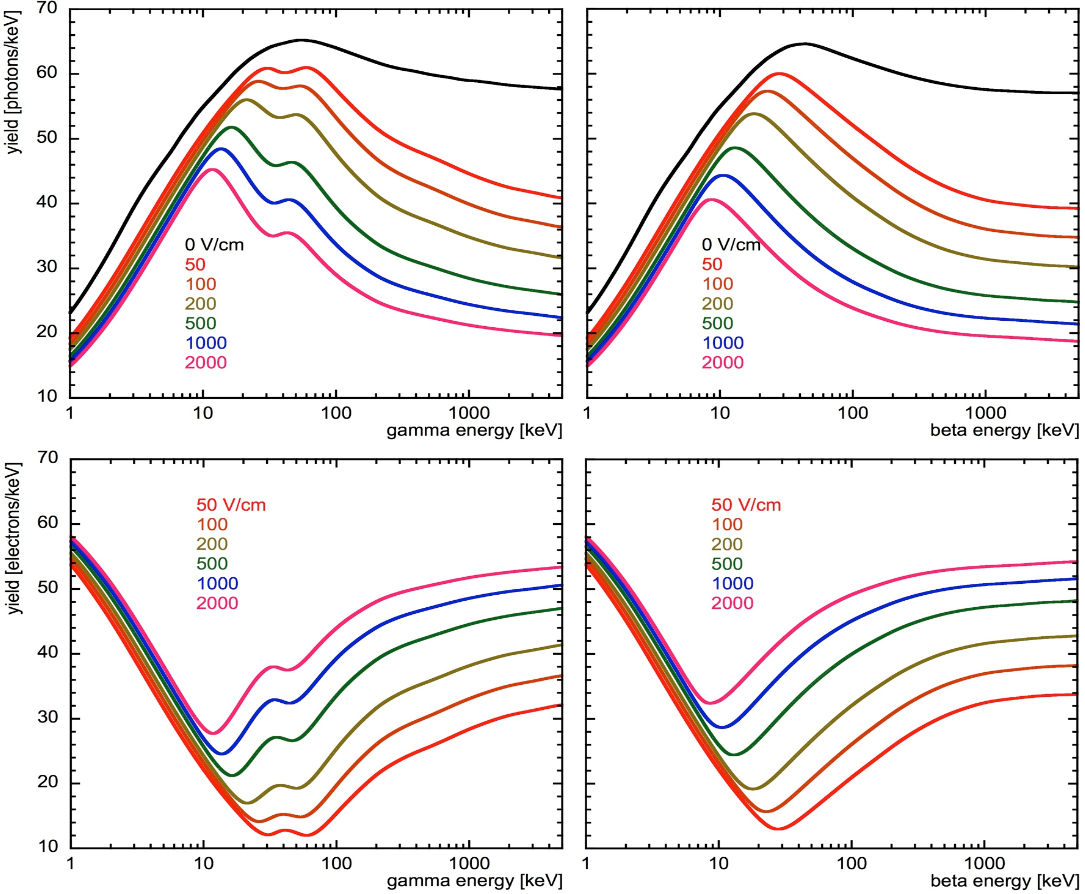
\includegraphics[scale=0.25]{figures/Recomb.png}
\captionof{figure}{Predictions from NEST for the light yield (top row) and charge yield (bottom row) of electron recoil event from gamma ray interaction (left column) and beta particle interaction (right column).  Field values are indicated by the colored lines.  Light yield and charge yield have less dependence on the field strength for lower energy events.  \cite{RecombSource} }
 \label{fig:LYQY}
\end{center}



\section{Signal Corrections in a Nonuniform Drift Field}\label{section:GenStrat}

In LUX's WS2014–16 data, pulse area corrections must account for field effects as a function of time, space, energy, and recoil type.  Since the recoil type of an event in WIMP search data is unknown, and the energy of an event in WIMP search data is unknown prior to pulse area corrections being applied, it is not possible to remove the spatial and time dependence induced by the field effects in our data.  Instead, we seek to separate the field effects from the detector inefficiency effects at the known energy and recoil type of $^{83m}$Kr, so that we can extract detector efficiency corrections that are applicable to all events from said data.  This separation must be performed at all points in time due to the time dependence of the electric field.  To accomplish this we relate the strength of the field effects in the S1 and S2 pulse areas of $^{83m}$Kr calibration data to the ratio of the two S1 pulses (referred to as S1a and S1b) generated during the $^{83m}$Kr decay.  This ratio is strongly correlated with the strength of the electric field, since the two $^{83m}$Kr decays have different energies (32.1 keV for S1a and 9.4 keV for S1b) and are therefore effected by the field effects by different amounts.  Note that corrections which perfectly separate field effects from detector inefficiency effects in this manner, and only correct for the latter, will have a spatial and time dependence left in the S1 and S2 signals but not in the energy spectra or gain factors for any data, regardless of energy or recoil type.

The general strategy for measuring and separating the electric field effects in $^{83m}$Kr calibrations is as follows.  First, we measure the electric field in the detector at a particular point in time, using the methods described in reference \ref{LuciesPaper}.  We would like to use this field map in conjunction with NEST to remove the field effects in the $^{83m}$Kr data directly before measuring detector inefficiency effects.  Unfortunately, due to the complicated nature of the $^{83m}$Kr decay NEST does not accurately simulate $^{83m}$Kr data.  Instead we turn to CH$_3$T data, which NEST has been tuned to simulate extremely well.  

After using NEST to determine and remove the strength of the field effects in CH$_3$T data we measure the residual pulse area variation in the S2 signal and produce corrections for these effects, which, since the field effects have been removed, are due to detector inefficiencies alone.  These detector inefficiency corrections are equivalent to the Run03 corrections which were obtained directly from $^{83m}$Kr data in~\cite{Run03Reanalysis}.  Next, we apply the detector inefficiency corrections to contemporaneous $^{83m}$Kr data.  At this point, any residual pulse are variation in the $^{83m}$Kr S2 signal is due to field effects alone.  We measure the strength of the field effects by fitting Gaussian distributions to the inefficiency corrected $^{83m}$Kr S2 signal over a three dimensional map, choosing the ratio S2(XYZ)/S2(Center) as the figure of merit for the strength of the field effect.  At the same time we measure a three dimensional map of the $^{83m}$Kr S1a/S1b ratio.  Relating these two maps allows us to determine the strength of the field effect on $^{83m}$Kr S2 data taken at any time or location by simply measuring the $^{83m}$Kr S1a/S1b ratio. 


The same process can not be repeated for the S1 signal, since the maximum of the CH$_3$T S1 spectrum falls below the detector threshold, and there are no discernible features to extract detector inefficiency corrections from.  Instead, three approaches have been taken to measure the relationship of the field effect in inefficiency corrected $^{83m}$Kr S1 data, as measured by S1(XYZ)/S1(Center), to the $^{83m}$Kr S1a/S1b ratio.  The first approach, in section \ref{section:S1relation}, converts the S2 field effect relationship to an S1 field effect relationship using the physics behind recombination.  In section \ref{MatthewsIdea} we use the expected light yield of the $^{83m}$Kr 31.2 keV decay as a function of electric field to measure detector inefficiency effects and separate them from the field effect we want to measure.  The final approach, in section \ref{section:S1relation2}, takes advantage of the fact that the energy spectrum of any event should remain insensitive to any recombination variation that arises from a non-uniform electric field.  In this method, we float the $^{83m}$Kr S1(XYZ)/S1(Center) to S1a/S1b relationship in a $\chi^2$ fit.  Within the fit we remove the field effect in both the S1 and S2 $^{83m}$Kr data (using the floated relationship for the S1 field effect), produce inefficiency-only corrections from the data, and then evaluate the corrected $^{83m}$Kr and CH$_3$T energy spectra.  The  S1(XYZ)/S1(Center) to S1a/S1b relationship which produces the minimum $\chi^2$ between the observed and expected energy spectra is chosen as the correct relationship.

Once the field induced S2(XYZ)/S2(Center) to S1a/S1b relationship and the field induced S1(XYZ)/S1(Center) to S1a/S1b relationship have been determined they can be used in $^{83m}$Kr data sets from any time to remove the field effects in the $^{83m}$Kr data via mapping the S1a/S1b ratio.  Once the field effects are removed the residual S1 and S2 variation in the $^{83m}$Kr can be used to calculate pulse area corrections based on detector inefficiencies alone. The following sections detail each step of the process outlined above.

\subsection{Measuring Detector Inefficiency Corrections with CH$_3$T}

The first step in measuring the strength of field effects in $^{83m}$Kr calibration data is to extract detector inefficiency corrections from contemporaneous CH$_3$T data.  We use data from the September 2015 CH$_3$T calibration due to its high statistics ($\sim$300,000 events). 

Before measuring detector inefficiency corrections from CH$_3$T, we must remove the field effects from the data.   The electric field at the location of each CH$_3$T event is estimated by interpolating the electric field map from~\cite{LuciesPaper}.  A cubic interpolation is used for events which fall within the bounds of the field map, and a nearest neighbor extrapolation is used for events which fall outside of the bounds.   

Once the field strength at the location of a particular event is determined it is converted to a measurement of the recombination for each event using the following equations from the NEST framework:
\begin{align}
N_q &= \frac{E}{0.0137} \label{NqEq} \\
N_{ion} &= \frac{N_q}{1+\alpha} \label{NionEq} \\
R &= 1-\mbox{ln} \left( \frac{1+(\frac{TI*N_{ion}}{4})}{(\frac{TI*N_{ion}}{4})} \right)
\end{align}
where $E$ is the energy of the event, $N_q$ is the number of quanta, $N_{ion}$ is the number of ions, $\alpha$ is the exciton to ion ratio (assumed to be 0.11), $TI$ is the Thomas-Imel Box parameter, and $R$ is the recombination probability.  Since we do not know the energy of the event ahead of time (since we do not have working corrections at this point) we assume the most probably energy from the CH$_3$T energy spectrum, which is 2.5 keV.  We are mainly interested in fitting the maximum of the spectrum when measuring detector inefficiency corrections, so the fact that this recombination estimate for higher energy CH$_3$T events may be wrong is not concerning.  

A normalization factor $N_{photon-center}/N_{photon}$ for the S1 signal is determined by calculating the number of photons produced in events at the center of the detector, and the number of photons produced in a particular event by using
\begin{equation}
N_{photon} = N_q\frac{\alpha}{1+\alpha} + N_{ion}R
\end{equation}
Since we assumed a value of 2.5 keV for all events, the normalization constant only has a dependence on the estimated field strength at each location in the detector.  

Similarly, we determine a normalization factor $N_{elec-center}/N_{elec}$ for the S2 signal by calculating the number of electrons at the center of the detector and the number of electrons for a particular event by using the equation
\begin{equation}
N_{elec}=N_q-N_{photon}
\end{equation}
which again is only dependent on the estimated field strength at each location in the detector.  

We multiply the raw S1 and S2 signals by these normalization factors to remove the field effects from the CH$_3$T data.  For clarity, we define the field effect removed S1 and S2 signals as S1$_F$ and S2$_F$, respectively, where the subscript $F$ stands for "field corrected".   
\begin{align}
S2_F &=S2 \left( \frac{N_{elec-center}}{N_{elec}} \right) \\
S1_F &=S1 \left( \frac{N_{photon-center}}{N_{photon}} \right)
\end{align}
Likewise, we define the detector inefficiency corrected S1 and S2 signals (with field effects still present) as S1$_E$ and S2$_E$, where the subscript $E$ stands for "efficiency corrected."

After removing the field effects from the CH$_3$T data we are ready to measure the residual spatial pulse area variation due to detector inefficiencies alone.  We first measure the Z dependence of the S2$_F$ pulse area by slicing the detector into drift time bins of 10 $\mu$second width.  A Landau distribution is fit to the S2$_F$ spectrum of each bin to determine the location of the spectra maximums.  A cubic interpolation is used to determine the S2$_F$ Z dependence between each drift time bin, and a linear extrapolation based on the first and last 20\% of data points is used to determine the S2$_F$ Z dependence above and below the span of the drift time bins.  A detector inefficiency correction for the Z direction, defined as $\epsilon_{(S2,Z)}$, is measured by taking the ratio of the S2$_F$ pulse area at a height of 4 $\mu$seconds (just below the liquid surface) to the S2$_F$ pulse area as described in the equation
\begin{equation}
\epsilon_{(S2,Z)}= \frac{S2_F(z=4)}{S2_F(z)}.
\end{equation} 


The XY dependence of the field removed S2$_F$ signal, defined as $\epsilon_{(S2,XY)}$, is found by dividing the Z inefficiency corrected (S2$_F \times \epsilon_{(S2,Z})$) data into two dimensional XY bins with lengths of 3 cm on each side, and then fitting Landau distributions to the data of each bin.  The maximum of the Landau distribution from each bin is used to construct an S2$_F$ XY dependence map, with a spline interpolation and extrapolation being used to determine the XY dependence between and outside of the bins.  A detector inefficiency correction for the XY direction is defined by taking the ratio of the z inefficiency corrected S2$_F$ pulse area at the center of the detector to the z inefficiency corrected S2$_F$ pulse area as a function of XY in cm, as shown below
\begin{equation}
\epsilon_{(S2,XY)} = \frac{\epsilon_{(S2,Z)} \times S2_F(x_c,y_c,z)} { \epsilon_{(S2,Z)} \times S2_F(xyz)}.
\end{equation} 
where $x_c$ and $y_c$ are the x and y center of the detector in uncorrected coordinates determined by taking the average position of the CH$_3$T events in each direction.



Multiplying the raw S2 signal by both the Z and the XY correction factors results in an inefficiency corrected S2$_E$ signal (with field effects still present), 
\begin{equation}\label{E_eq}
S2_E =S2 \times \epsilon_{(S2,Z)} \times \epsilon_{(S2,XY)} 
\end{equation}

We are unable to directly measure the detector inefficiency corrections for the S1 signal from CH$_3$T data, since the maximum of the S1 spectrum falls below the detector threshold and there are no discernible features to fit to. Instead, we will continue working with the S2 signal of our data and return to the issue of S1 corrections in sections \ref{section:S1relation,MatthewsIdea,section:S1relation2}.


 
\subsection{Measuring Field Effects in $^{83m}$Kr S2 Data} \label{section:FieldEffects}

After measuring the S2 detector inefficiency corrections in CH$_3$T data we have all the tools we need to measure the field effects in the S2 pulse area of $^{83m}$Kr data.  We begin by applying the S2 detector inefficiency corrections to contemporaneous,  uncorrected $^{83m}$Kr data by using equation \ref{E_eq}.  The removal of the detector inefficiency effects from the raw S2 data leave us with an S2$_E$ signal which has spatial pulse area variation from field effects alone.

The process for measuring the field effects in the inefficiency corrected $^{83m}$Kr S2$_E$ data is similar to the process of measuring the detector inefficiency effects in the field effect corrected CH$_3$T S2$_F$ data.  First, we measure the field induced Z dependence of the $^{83m}$Kr S2$_E$ pulse area by slicing the detector into drift time bins of 10 $\mu$second width.  A Gaussian distribution is fit to the S2$_E$ spectrum of each bin to determine the mean S2$_E$ pulse area versus Z.   A cubic interpolation is used to determine the S2$_E$ Z dependence between each drift time bin, and a linear extrapolation based on the first and last 20\% of data points is used to determine the S2$_E$ Z dependence above and below the span of the drift time bins.  

We define the strength of the field effect in the z direction as the ratio of the S2$_E$ pulse area as a function of Z to the S2$_E$ pulse area at the center of the detector $z_c$, S2$_E$(z)/S2$_E$(center).  An S2 field effect correction for the Z direction, defined as $\eta_{(S2,Z)}$, is measured by taking the inverse of the strength of the field effect, 
\begin{equation}
\eta_{(S2,Z)} = \frac{S2_E(z=z_c)}{S2_E(z)}.
\end{equation} 

We also take a separate, three dimensional approach to mapping the field effect in the $^{83m}$Kr S2$_E$ data. In this approach the detector is divided into three dimensional voxels, with X and Y width of 3.5 cm and Z width of 30 $\mu$seconds.  As in the one dimensional case, a three dimensional map of the field induced S2$_E$ pulse area variation is produced by fitting a Gaussian distribution to the $^{83m}$Kr S2$_E$ data in each voxel.  A spline interpolation is used to determine the S2$_E$(xyz)/S2$_E$(center) ratio between the three dimensional voxels, and the S2$_E$(xyz)/S2$_E$(center) Z dependence map is used to extrapolate outside of the range of the voxels.  As shown in Figure~\ref{fig:S1aS1bField_S2}, the results are consistent between both measurements.

\subsection{Measuring the S1a and S1b Pulse Areas in $^{83m}$Kr data} \label{section:S1aS1b1}

Once we have measured the strength of the field effect from the $^{83m}$Kr S2$_E$ data at one point in time, we need to develop a method to track the field effect at all points in time.  To accomplish this, we use the uncorrected S1 pulse area from the 32.1 keV and 9.4 keV decays within $^{83m}$Kr events, referred to as S1a and S1b respectively.  As discussed in section \ref{section:Intro}, as the electric field increases the probability of recombination decreases, leading to a smaller S1 signal.  The S1a decay is more sensitive to this effect due to its higher energy, leading to a stronger field effect in the S1a data than in the S1b data.   Therefore, an inverse relationship exists between the strength of the field and the S1a/S1b ratio.  

To measure the size and location of the S1a and S1b decays, we select $^{83m}$Kr events with an S2 pulse area pulse area between 2000 to 60000 phe as measured by the bottom PMT array.  We identify S1 candidates that have pulse area above 10 phe, such that each $^{83m}$Kr event is defined to have exactly one candidate S2 and at least one candidate S1.  After the event selection is complete, a region of interest (ROI) beginning at the first candidate S1 and ending at the start of the S2 (or after 150 samples) is defined. The ROI is then used to select sumpod data from the evt files within the ROI.  This data is  fit to a double exponential function which returns the pulse area and maximum fractional area of the S1a and S1b peaks, as well as the time separation between them (Figure~\ref{fig:Sumpod}). We can not produce reasonable fits for events in which the S1a and S1b decays are separated by less than 130 nanoseconds, so a cut requiring the separation between S1a and S1b events to be great than this is applied  (Figure~\ref{fig:S1aS1btiming}).

\begin{figure}
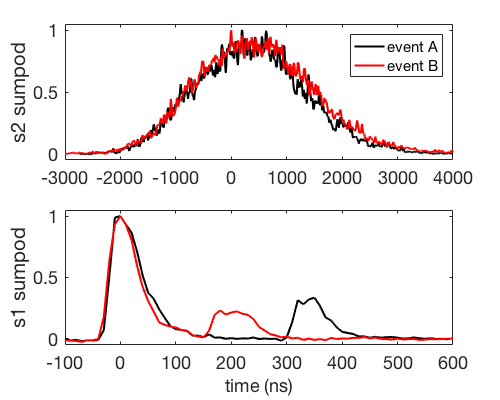
\includegraphics[scale=0.4]{figures/S1abS2_sumpod_040317_2.png}
\captionof{figure}{Sumpod versus time for a $^{83m}$Kr in which a distinct S1a and S1b peak have been observed. In this case, the fit finds an S1a area of 174 phe, an S1b area of 64.5 phe, and a separation in time of 35 samples.}
 \label{fig:Sumpod}
\end{figure}

\begin{figure} [!h]
\centering
\subfloat{{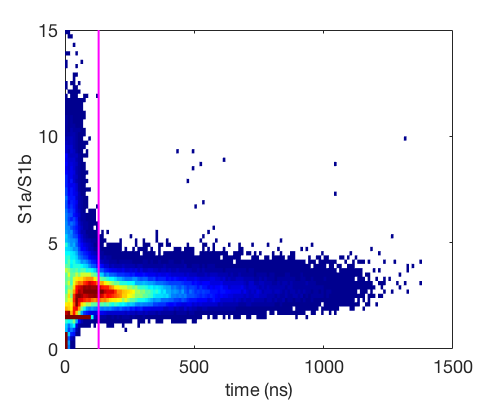
\includegraphics[width=7cm]{figures/S1aS1bCut_Timing_1.png} }}
\qquad
\subfloat{{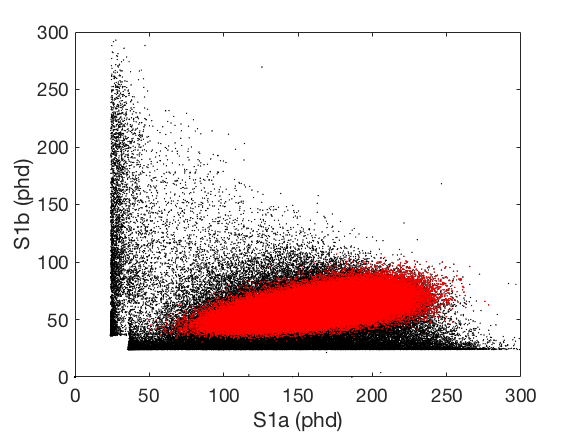
\includegraphics[width=7cm]{figures/S1aS1bCut.png} }}
\caption{ (Top) The output of the S1a/S1b fitting module as a function of time separation between the two decays.  The red line indicate the minimum separation between the S1a and S1b events required by our cut in this analysis. (Bottom) A scatter plot of all S1a and S1b pulse areas measured by the fitting module (black) compared to the S1a and S1b pulse areas that are left after our selection cut. (red)}
\label{fig:S1aS1btiming}
\end{figure}

\subsection{Relating the S1a/S1b Ratio to S2 Field Effects} \label{section:S1aS1b2}

To relate the S1a/S1b ratio to the S2 field effects measured in section \ref{section:FieldEffects} we begin by measuring the spatial dependence of the S1a/S1b ratio.  We first divide the detector into drift time bins of 3 $\mu$second width.   A Gaussian distribution is fit to the S1a and S1b spectrum of each bin to determine the mean pulse areas versus Z.   A second order polynomial is fit to the ratio of the Gaussian means versus Z and is used to determine the S1a/S1b ratio at any drift time in the detector.  

As we did when measuring the strength of the field effect, we also take a separate, three dimensional approach to mapping the $^{83m}$Kr S1a/S1b ratio throughout the detector. In this approach the detector is divided into three dimensional voxels, with X and Y width of 3.5 cm and Z width of 30 $\mu$seconds.  A three dimensional map of S1a/S1b is produced by fitting a Gaussian distribution to the S1a and S1b pulse area spectrum in each voxel.  A spline interpolation and extrapolation is used to determine the S1a/S1b ratio between and outside of the three dimensional voxels.

We relate the Z dependence and three dimensional dependence maps of the S1a/S1b ratio to the Z dependence and three dimensional dependence maps of the S2 field effect measured in section \ref{section:FieldEffects}.  A second order polynomial is fit to the spatial dependence of the $^{83m}$Kr S2$_E$ (induced by the field effect) to S1a/S1b relationship, with best fit parameters of $a=-0.499 \pm 0.117$,$b=1.48 \pm 0.615$, and $c=0.667 \pm 0.946$ for the second order, first order, and zeroth order terms, respectively. This polynomial is used to determine the strength of the field effect in $^{83m}$Kr S2 data at all points in time.  We find that the Z dependence and three dimensional maps agree closely within the range of measured S1a/S1b ratios, but begin to diverge in the extrapolated regions (Figure \ref{fig:S1aS1bField_S2}). 

\begin{center}
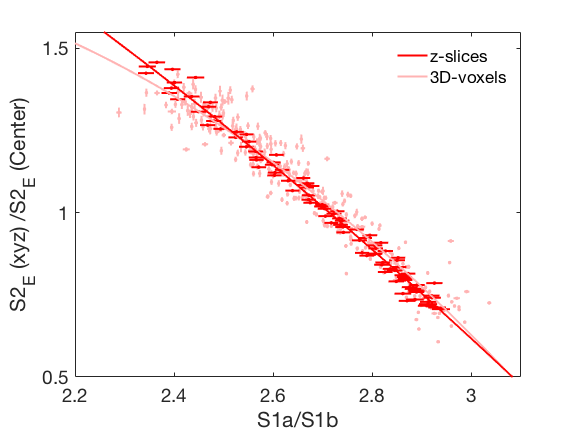
\includegraphics[scale=0.4]{figures/S1aS1bvField_ZDep_3D_S2Only.png}
\captionof{figure}{The Z (dark red) and three dimensional (light red) relationship of the $^{83m}$Kr S1a/S1b ratio to the $^{83m}$Kr S2$_E$ field effect.}
 \label{fig:S1aS1bField_S2}
\end{center}

\subsection{Measuring the S1a/S1b Ratio to S1 Field Effect Relationship with Recombination Physics} \label{section:S1relation}

We have successfully measured the strength of the field effect in $^{83m}$Kr S2 data at one point in time, and have related it to the $^{83m}$Kr S1a/S1b ratio such that we can determine the strength of the field effect at any point in time.  We are now left with the challenge of measuring the strength of the field effect in $^{83m}$Kr S1 data. Our first approach will turn to the recombination physics that governs particle interaction during a recoil event.  

The strength of the field effect (normalized to the detector center) in $^{83m}$Kr S2 data is given by the ratio of the inefficiency corrected S2$_E$ at a given position to the inefficiency corrected S2$_E$ at the center of the detector, which was measured in \ref{section:FieldEffects}.  This ratio can be written in terms of the recombination during a $^{83m}$Kr event ($R_{Kr}$) as follows
\begin{equation}
\frac{S2_{E,Kr}(xyz)}{S2_{E,Kr}(center)} = \frac{1-R_{Kr}(xyz)}{1-R_{Kr}(center)}
\end{equation}
Note that this can be rewritten as an expression for the recombination during a $^{83m}$Kr as a function of position,
\begin{equation} \label{RKr}
R_{Kr}(xyz) = 1- \frac{S2_{E,Kr}(xyz)}{S2_{E,Kr}(center)}(1-R_{Kr}(center)).
\end{equation}
Next, we write the strength of the field effect in $^{83m}$Kr S1 data (normalized to the detector center) as the ratio of the inefficiency corrected S1$_E$ signal at a given position to the inefficiency corrected S1$_E$ signal at the center of the detector, which we are unable to measure directly.  In terms of the exciton to ion ratio ($\alpha$) and the recombination during a $^{83m}$Kr event this is given by 
\begin{multline} \label{S1fieldstrength}
\frac{S1_{E,Kr}(xyz)}{S1_{E,Kr}(center)}=\frac{\alpha+R_{Kr}(xyz)}{\alpha+R_{Kr}(center)} \\ = \frac{\alpha + 1 - \frac{S2_{E,Kr}(xyz)}{S2_{E,Kr}(center)}(1-R_{Kr}(center))}{\alpha + R_{Kr}(center)}
\end{multline}
where we have used equation \ref{RKr} in the last step.  Therefore, all we need to measure the strength of the field effect in $^{83m}$Kr S1 data is the recombination during a $^{83m}$Kr event at the center of the detector, given by $R_{Kr}(center)$.  As mentioned in section \ref{section:GenStrat}, NEST does not simulate the physics of $^{83m}$Kr events well, but it has been tuned to simulate the physics of CH$_3$T events.  As such, we once again turn to the CH$_3$T data to determine the value of $R_{Kr}(center)$. 

First, we write the ratio of the efficiency corrected $^{83m}$Kr  S2$_E$ pulse area at the center of the detector to the efficiency corrected CH$_3$T S2$_E$ pulse are at the center of the detector in terms of the S2 gain factor ($g_2$), recombination during a $^{83m}$Kr event ($R_{Kr}$), recombination during a CH$_3$T event ($R_{H3}$), number of ions produced during a $^{83m}$Kr event ($N_{ion-Kr}$), and number of ions produced during a CH$_3$T event ($N_{ion-H3}$), given by
\begin{equation}
\frac{S2_{E,Kr}(center)}{S2_{E,H3}(center)} = \frac{g_2(1-R_{Kr}(center))N_{ion-Kr}}{g_2(1-R_{H3}(center))N_{ion-H3}}.
\end{equation}
This can be rewritten as an expression for the recombination of $^{83m}$Kr at the center of the detector given by
\begin{multline} \label{RKr_cent}
R_{Kr}(center)=1- \\ \frac{S2_{E,Kr}(center)}{S2_{E,H3}(center)}\frac{N_{ion-H3}}{N_{ion_Kr}}(1-R_{H3}(center))
\end{multline}
where the gain factor $g_2$ does not depend on energy, and therefore can be removed from the equation.  The number of ions for both $^{83m}$Kr events and CH$_3$T events is given by equations \ref{NqEq} and \ref{NionEq}, with the assumption $E=41.55$ keV for $^{83m}$Kr and $E=2.5$ keV for CH$_3$T, and the recombination at the center of the detector of CH$_3$T events ($R_{H3}$) can be determined from NEST.

Using equations \ref{S1fieldstrength} and \ref{RKr_cent} we can convert the field effect measured in the $^{83m}$Kr S2$_E$ data to an inferred field effect in $^{83m}$Kr S1 data.
The result of this is shown in Figure \ref{fig:S1FieldFig}.  It is possible that the complicated nature of the  $^{83m}$Kr decay introduces intricacies which are not account for in equations \ref{S1fieldstrength} and \ref{RKr_cent}.  In the next section we will seek to improve this result with a direct measurement of the S1a/S1b to S1 field effect relationship before turning to a $\chi^2$ minimization method in section \ref{section:S1relation2} to determine the optimal field effect to S1a/S1b relationships.


\begin{figure}
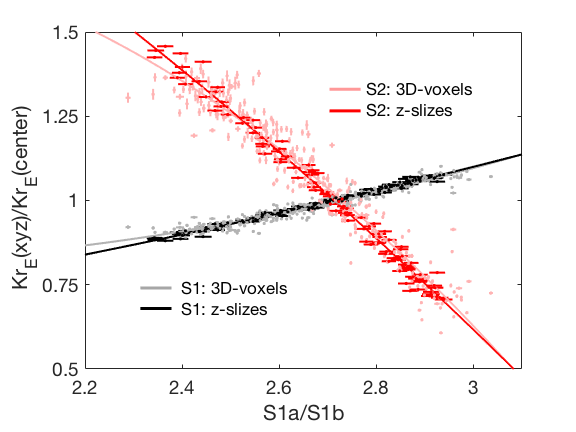
\includegraphics[scale=0.4]{figures/S1aS1bvField_ZDep_3D.png}
\captionof{figure}{The Z (black) and three dimensional (grey) relationship of the $^{83m}$Kr S1a/S1b ratio to the $^{83m}$Kr S1 field effect.  The black and grey data points are not measured, but instead inferred from the Z (dark red) and three dimensional (light right) relationship of the $^{83m}$Kr S1a/S1b ratio to the $^{83m}$Kr S2$_E$ field effect.}
 \label{fig:S1FieldFig}
\end{figure}

\subsection{Measuring the S1a/S1b Ratio to S1 Field Effect Relationship with the S1a Light Yield} \label{MatthewsIdea}

The relative light yield of the $^{83m}$Kr 32.1 keV decay, $^{83m}$Kr 9.4 keV decay, and $^{57}$Co 122 keV decay has been measured as a function of the light yield at an applied electric field divided by the light yield at zero electric field by Manalaysay, et al. in reference \cite{Manalaysay}.  We can combine NEST predictions for the light yield of the 122 keV $^{57}$Co line with the ratio of the light yield of the 32.1 keV $^{83m}$Kr line to the 122 keV $^{57}$Co line from reference \cite{Manalaysay} to convert the relative light yield measurements to absolute light yield measurements.  This results in an empirical formula for the absolute light yield of the $^{83m}$Kr 32.1 keV decay as a function of electric field given by
\begin{equation}
\frac{\gamma}{E} = 55.2[1-0.0004895 \times F \times \ln{(1 + 1/(8.9\mathrm{e}{-4} \times F))}]
\label{S1aYield}
\end{equation}
where $\gamma$ is the number of photons, $E$ is the energy of the decay, and $F$ is the applied electric field in units of V/cm.  

Using equation \ref{S1aYield} we can directly measure the strength of the field effect in the $^{83m}$Kr S1 data and relate it to the S1a/S1b ratio.  We begin by using the electric fields maps presented in reference~\cite{LuciesMaps} to estimate the electric field in the detector in September 2015.   The electric field map is converted to a map of the expected light yield at 32.1 keV using equation \ref{S1aYield}, assuming no detector inefficiency effects are present. The three dimensional spatial dependence of the light yield provides a direct measurement of the strength of the field effect in the S1a data, given by $\gamma(xyz)$/$\gamma(center)$.  Note that the strength of the field effect in the S1a data can help us derive the strength of the field effect in the combined S1 data, but the two are not equivalent.  Normalizing the field effect in the S1a data to the center of the detector, as shown in equation \ref{S1aNorm}, produces S1a$_F$ data which has spatial variation due to detector inefficiency effects only.  
\begin{equation}
S1a_F = S1a \frac{\gamma(center)}{\gamma(xyz)}
\label{S1aNorm}
\end{equation}
We measure the detector inefficiency effects in the S1a$_F$ data by dividing the detector into three dimensional voxels with X and Y width of 7 cm and Z width of 47 $\mu$Sec.  A Gaussian distribution is fit to the S1a$_F$ spectrum in each voxel, and the Gaussian mean is used to determine the spatial dependence of the S1a$_F$ data due to detector inefficiency effects alone.  Since the detector inefficiency effects are not dependent on the energy of an event, the spatial variation measured in the S1a$_F$ data is equivalent to the spatial variation in the combined S1 data due to detector inefficiency effects alone.  Therefore, we can use the spatial variation measured in the S1a$_F$ data to produce detector inefficiency corrected combined S1$_E$ data as shown in the equation
\begin{equation}
S1_E= S1 \frac{S1a_F(center)}{S1a_F(xyz)}.
\end{equation}
Any residual spatial variation in the detector inefficiency corrected combined S1$_E$ data is due to field effects in the combined $^{83m}$Kr S1 data alone.  We measure the strength of these field effects by again dividing the detector into three dimensional voxels with X and Y width of 7 cm and Z width of 47 $\mu$Sec.  A Gaussian distribution is fit to the S1$_E$ spectrum in each voxel, and the Gaussian mean is used to determine the spatial dependence of the S1a$_E$ data due to field effects alone.  At the same time, we use separate Gaussian distribution fits to the S1a and S1b data in each voxel to measure the spatial dependence of the S1a/S1b ratio.  Finally, we relate the S1a$_E$ Gaussian mean to the S1a/S1b ratio of each voxel and fit a second order polynomial which describes the strength of the field effect in the $^{83m}$Kr combined S1 signal to the data. (Figure \ref{S1aFieldEffect}) Note that the large systematic errors in the S1a/S1b ratio to field effect relationship is introduced by uncertainties in the field maps and systematic errors in the detector inefficiency corrections.  These errors a significantly reduced when extracting efficiency corrections from CH$_3$T data due to the lower energy, and therefore lower sensitivity to field effects.

\begin{minipage}{8.15cm}
\begin{center}
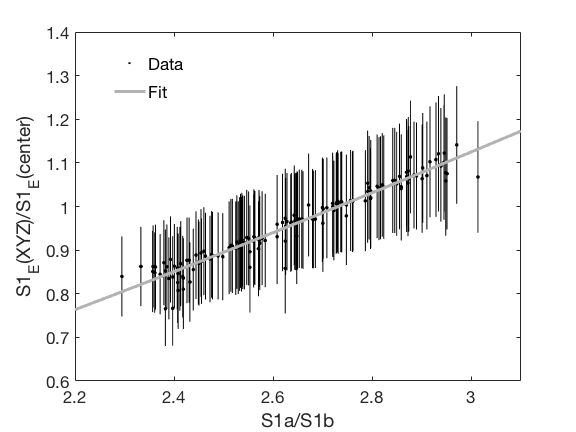
\includegraphics[scale=0.4]{figures/MatthewS1FieldEffectMeasurement.png}
\captionof{figure}{The strength of the S1 field effect measured in this section (grey) compared to the strength of the S1 field effect measured in section \ref{section:S1relation2} (blue).  The large error bars on the data are due to systematic uncertainties in the field maps detector inefficiency corrections.}
\label{S1aFieldEffect}
\end{center}
\end{minipage}

\subsection{Measuring the S1a/S1b Ratio to S1 Field Effect Relationship with a $\chi^2$ Fitting Method} \label{section:S1relation2}

Although field induced variation in the recombination of a $^{83m}$Kr event can introduce a spatial and time dependence in the $^{83m}$Kr S1 and S2 signals, the total energy signal given (with gain factors $g_1$ and $g_2$) by 
\begin{equation} \label{CombinedEnergy}
E=\left(\frac{1}{73}\right)\left(\frac{S1_E}{g_1} + \frac{S2_E}{g_2}\right)
\end{equation}
should be insensitive to field variations.  We can take advantage of this fact to determine the optimal S1a/S1b to S1 field effect relationship corresponding to the directly measured S1a/S1b to S2 field effect relationship measured in section \ref{section:S1aS1b2}.  Unfortunately, we do not have knowledge of the strength of the field effect in the $^{83m}$Kr S1 signal, so we can not remove the field effect from the data to produce the efficiency-only corrected S1$_E$ signal.  Likewise, without efficiency corrected data we can not measure the gain factors $g_1$ and $g_2$ to produce a combined energy spectrum.  The only tools that we have at our disposal are a measurement of the strength of the field effect in the $^{83m}$Kr S2 signal and its relationship to S1a/S1b, as well as the ability to produce efficiency only corrected $^{83m}$Kr S2$_E$ data based on to the spatial variation of field effect corrected  $^{83m}$Kr S2$_F$ data.  In this section we turn to a $\chi^2$ minimization approach which will float the S1 field effect to S1a/S1b relationship, produce inefficiency corrections based on the field removed S1$_F$ and S2$_F$ signals, and then float the gain factors $g_1$ and $g_2$ to produce an optimized combined energy spectrum.  

We begin by eliminating one of the three parameters associated with the second order polynomial which describes the S1 field effect to S1a/S1b relationship.  We choose to normalize the spatial variation induced by the nonuniform electric field to the center of the detector, so the strength of the field effect as measured by $\frac{S1_{E,Kr}(xyz)}{S1_{E,Kr}(center)}$ must equal one at the center of the detector.  Therefore, we can relate one of the coefficients ($a$,$b$, and $c$) in the second order polynomial
\begin{equation}
 \frac{S1_{E,Kr}(xyz)}{S1_{E,Kr}(center)} = a\left(\frac{S1a}{S1b}\right)^2 + b\left(\frac{S1a}{S1b} \right) + c
 \end{equation}
 to the other two, such that
 \begin{equation}
 c=1-a\left(\frac{S1a_c}{S1b_c}\right)^2-b\left(\frac{S1a_c}{S1b_c}\right)
 \end{equation}
 where $S1a_c$ and $S1b_c$ represent the values of $S1a$ and $S1b$ at the center of the detector.  Next, we scan over a range of $a$ and $b$ values and produce the $\frac{S1_{E,Kr}(xyz)}{S1_{E,Kr}(center)}$ to $\frac{S1a}{S1b}$ relationship for each pair of $a$ and $b$ values.  We follow the procedure described in section \ref{KrypCalCode} and use the S1 field effect to S1a/S1b relationship from each pair of $a$ and $b$ values, in conjunction with the S2 field effect S1a/S1b relationship measured in \ref{section:FieldEffects}, to produce efficiency-only corrections for CH$_3$T data and $^{83m}$Kr data from September 2015 and February 2016. These corrections are used to produce S2$_E$ and S1$_E$ data for all four data sets.  We then scan over a range of $g_1$ and extraction efficiency (EE) values and use the S2$_E$ and S1$_E$ data to produce a combined energy spectrum (for each source) for each combination of $a$,$b$,$g_1$, and EE based on equation \ref{CombinedEnergy}.  Note that $g_2=SE \times EE$, where $SE$ is the single electron size at the time of each data set.  

To evaluate the performance of each $a$,$b$,$g_1$, and $EE$ combination we must develop models for the expected energy spectra of CH$_3$T and $^{83m}$Kr data in September 2015 and February 2016.  The $^{83m}$Kr events consist of a mono-energetic 32.1 keV decay and a mono-energetic 9.4 keV decay.  The expected energy spectrum is a Gaussian distribution centered around the sum of these two mono-energetic decays at 41.55 keV.  The width of the Gaussian distribution depends on a number of factors, including the detector's efficiency for collecting S1 and S2 light, as well as the spatial dependence of the recombination of $^{83m}$Kr events induced by the nonuniform electric field.  While we can measure most of these parameters, we would have to feed them into NEST to determine the final width of the Gaussian distribution.  Since NEST does not simulate $^{83m}$Kr events well, we can only use the mean of the Gaussian distribution as a figure of merit for the $^{83m}$Kr energy spectrum.

Tritium is a beta decay with an energy spectrum that has a broad peak at 2.5 keV and a smoothly falling distribution out to 18 keV.  As with $^{83m}$Kr, this spectrum is smeared based on a number of parameters.  Unlike $^{83m}$Kr, the smearing in CH$_3$T data can be accurately determined by NEST so we can compare the energy spectrum from data to simulations on a bin by bin basis. 

For each $a$,$b$,$g_1$, and $EE$ combination a reduced $\chi^2$ for the CH$_3$T and $^{83m}$Kr data is measured using the difference between the expected energy spectra and measured energy spectra.   During the $^{83m}$Kr $\chi^2$ calculation, the energy spectrum is from each point in time is divided into drift time bins so that the spatial dependence of the energy spectrum is included in the $\chi^2$ measurement.  The $^{83m}$Kr data has very high statistics, and only the mean of a Gaussian fit to the data is of interest, so the variance used in the $\chi^2$  measurement  is dominated by systematic error.  We use the standard deviation of the $^{83m}$Kr energy spectrum over the duration of Run03 to evaluate the size of this systematic error, and find $\sigma = 0.2395$.  During the CH$_3$T $\chi^2$  calculation, the energy spectrum is divided into energy bins so that the entire beta spectrum (above 3.5 keV to avoid the detector threshold) is included in the $\chi^2$ measurement.  The variance of the CH$_3$T data is based on statistics alone, due to finer binning and lower statistics of the data.  We choose to define a total reduced $\chi^2$ (to be minimized in the $\chi^2$ fit) as the average of the reduced $\chi^2$ for the $^{83m}$Kr and CH$_3$T data, so that each source carries the same amount of weight in the fit. A minimum average reduced  $\chi^2$ of 0.8413 is found for the best fit parameters of $a=0.065 \pm 0.0117$,$b=0.020 \pm 0.060$,$g_1=0.0980 \pm 0.001$, and $EE=0.808 \pm 0.029$. The corresponding value of the zeroth order coefficient is $c=0.461 \pm 0.186$.  The reduced $\chi^2$ of the $^{83m}$Kr and CH$_3$T energy spectra separately are 12.17/26=0.4682 (p=0.99) and 150.6/124=1.2143 (p=0.05), respectively. Note that (as we will see in section \ref{Results}) the extraction efficiency needed to produce these results is consistent with our expectations, and the results produce $^{83m}$Kr energy peaks (unbinned in drift time) that are within one sigma of the expected 41.55 keV in both September 2015 and February 2016. 


\subsection{Summary of S1a/S1b Ratio to Field Effect Measurements}

We have directly measured the strength of the field effect in $^{83m}$Kr S2 data by removing detector inefficiency effects from the data with the help of CH$_3$T data.  We have also used a $\chi^2$ optimization methods to find the optimal S1 field effect to S1a/S1b relationship to pair with the direct S2 field effect measurement.  We find that the optimal S1 field effect found by a $\chi^2$ optimization agrees very closely with our expectations from recombination physics, and from the expected light yield of the $^{83m}$Kr S1 data 32.1 keV decay.   We choose to use the S2 field relationship measured in section \ref{section:S1aS1b2} and the corresponding optimal S1 field effect relationship measured in section \ref{section:S1relation2} for our work.  The polynomials that describe these relationships are:
\begin{multline}
\frac{S2_{E,Kr}(xyz)}{S2_{E,Kr}(center)} =   \\ -0.499 \left(\frac{S1a}{S1b} \right)^2 + 1.48  \left(\frac{S1a}{S1b} \right) + 0.667
\end{multline}
\begin{multline}
\frac{S1_{E,Kr}(xyz)}{S1_{E,Kr}(center)} = \\  0.065 \left(\frac{S1a}{S1b} \right)^2 + 0.020 \left(\frac{S1a}{S1b} \right) + 0.461
\end{multline}


\begin{center}
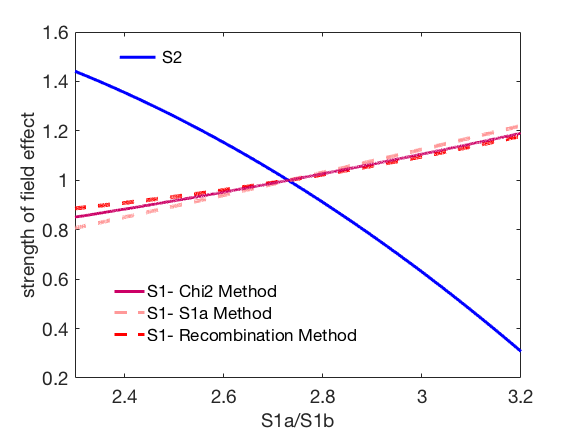
\includegraphics[scale=0.4]{figures/StrengthOfFieldEffectOverlay.png}
\captionof{figure}{The S1a/S1b to field effect relationships measured in this work.  The method to measure each line is indicated by the color in the legend.  Red shades indicate measurements of the strength of the field effect in  $^{83m}$Kr S1 data, and blue shades indicate the strength of the field effect in  $^{83m}$Kr S2 data. Solid lines represent measurements that are used in KrypCal, and dashed lines represent measurements that are supplementary cross checks. }
 \label{AllMeasurements}
\end{center}





\section{Producing Detector Inefficiency Corrections} \label{KrypCalCode}

Now that we have related the strength of the field effect in both $^{83m}$Kr S2 and $^{83m}$Kr S1 data to the S1a/S1b ratio we can make use of these relationships to produce detector inefficiency corrections during every $^{83m}$Kr calibration.  This process is very similar to (and in some ways, the reverse of) the process to measure the field effect in $^{83m}$Kr S2 data. Nevertheless, we will describe the process here for completeness and clarity.

\subsection{Mapping S1a/S1b}

For a $^{83m}$Kr calibration at any point in time, we begin by measuring the Z dependence of the S1a/S1b ratio using the methods of section  \ref{section:S1aS1b1} and  \ref{section:S1aS1b2}.  We first divide the detector into drift times bins with a width chosen such that each bin has roughly 300 events.   A Gaussian distribution is fit to the S1a and S1b spectrum of each bin to determine the mean pulse areas versus Z.  A second order polynomial is fit to the ratio of the Gaussian means versus Z and is used to determine the S1a/S1b at any drift time in the detector.  

If the $^{83m}$Kr data set has more than 100,000 S1a/S1b events (after cuts are applied) a three dimensional S1a/S1b map is also constructed. The detector is divided into three dimensional voxels with dimensions chosen such that each voxel has roughly 200 events.  A three dimensional map of S1a/S1b ratio is produced by fitting a Gaussian distribution to the S1a and S1b pulse area spectrum in each voxel.  A spline interpolation is used to determine the S1a/S1b ratio between the three dimensional voxels, and the S1a/S1b Z dependence map is used to extrapolate outside of the range of the voxels. 

\subsection{Removing the field effect from $^{83m}$Kr Data}

We use the $^{83m}$Kr S2 field effect to S1a/S1b relationship and S1 field effect to S1a/S1b relationship measured in sections \ref{section:FieldEffects} and \ref{section:S1relation2} to convert the Z and three dimensional maps of S1a/S1b into measures of the field effects in the S1 and S2 data.  The strength of the field effect is measured by $\frac{S1_E(xyz)}{S1_E(center)}$ and $\frac{S2_E(xyz)}{S2_E(center)}$.  Dividing the raw $^{83m}$Kr data by the strength of the field effect normalizes any field induced recombination variation to the level of recombination that occurred at the center of the detector, at the time the field effect relationships were measured.  This is equivalent to normalizing electric field in the $^{83m}$Kr data to it's value at the center of the detector in September 2015. Applying these normalization factors produces field effect corrected S1$_F$ and S2$_F$ signals, as shown in equations \ref{S1F-2} and \ref{S2F-2}. (Figure \ref{fig:KrypCalLifetime})
\begin{align} 
S1_F &=S1 \times \frac{S1_E(center)}{S1_E(xyz)} \label{S1F-2} \\
S2_F &=S2 \times \frac{S2_E(center)}{S2_E(xyz)} \label{S2F-2}
\end{align}

\subsection{Measuring Detector Inefficiencies}

After removing the field effects from the $^{83m}$Kr data we are ready to measure the residual spatial pulse area variation due to detector inefficiencies alone.  We first measure the Z dependence of the S2$_F$ and S1$_F$ pulse areas by slicing the detector into drift time bins with widths defined such that each bin has roughly 300 events.  A Gaussian distribution is fit to the S2$_F$ and S1$_F$ spectra of each bin to determine the location of the spectra maximums. (Figure \ref{fig:KrypCal_S2ZDep} and Figure \ref{fig:KrypCal_S1ZDep}) In the case of the S2$_F$ signal, a cubic interpolation is used to determine the S2$_F$ Z dependence between each drift time bin, and a linear extrapolation based on the first and last 20\% of Gaussian distribution data points is used to determine the S2$_F$ Z dependence above and below the span of the drift time bins.  A detector inefficiency correction for the Z direction is defined by taking the ratio of the S2$_F$  pulse area at a height of 4 $\mu$seconds (just below the liquid surface) to the S2$_F$ pulse area as a function of Z as described in the equation
\begin{equation}
\epsilon_{(S2,Z)} = \frac{S2_F(z=4)}{S2_F(z)}.
\end{equation} 

In the case of the S1$_F$ signal, a second order polynomial is used to determine the S1$_F$ Z dependence between and outside of each drift time bin. A detector inefficiency correction for the Z direction is defined by taking the ratio of the S1$_F$  pulse area at the center of the detector ($z_c$ as defined by the average drift time of $^{83m}$Kr) to the S1$_F$ pulse area as a function of Z as described in the equation
\begin{equation}
\epsilon_{(S1,Z)} = \frac{S1_F(z_c)}{S1_F(z)}.
\end{equation} 


The XY dependence of the field removed S2$_F$ and S1$_F$ signals are found by dividing the z inefficiency corrected (S2$_F \times \epsilon_{(S2,Z)}$ and S1$_F \times \epsilon_{(S1,Z)}$) data into two dimensional XY bins with lengths defined such that each bin has roughly 300 events, and then fitting Gaussian distributions to the data of each bin.  The mean of the Gaussian distribution from each bin is used to construct S2$_F$ and S1$_F$ XY dependence maps, with a spline interpolation and extrapolation being used to determine the XY dependence between and outside of the bins.  A detector inefficiency correction for the XY direction is defined by taking the ratio of the z inefficiency corrected S2$_F$ (or S1$_F$) pulse area at the center of the detector to the z inefficiency corrected S2$_F$ (or S1$_F$) pulse area as a function of XY in cm, as shown below
\begin{align}
\epsilon_{(S2,XY)} &= \frac{\epsilon_{(S2,Z)} \times S2_F(x_c,y_c,z)}{\epsilon_{(S2,Z)} \times S2_F(xyz)} \\
\epsilon_{(S1,XY)} &= \frac{\epsilon_{(S1,Z)}\times S1_F(x_c,y_c,z)}{\epsilon_{(S1,Z)} \times S1_F(xyz)}.
\end{align} 
where $x_c$ and $y_c$ are the x and y center of the detector in uncorrected coordinates determined by taking the average position of the $^{83m}$Kr events in each direction.  

To apply these S1 and S2 efficiency corrections to data at any time, we must interpolate between the corrections in time.  The S2$_E$ XY, S1$_E$ Z, and S1$_E$ XY efficiency corrections are not expected to change rapidly in time, so a simple nearest neighbor interpolation is used to apply these efficiency corrections to data sets at any point in time.  However, the S2$_E$ Z dependence is expected to change rapidly in time due to the sudden changes in xenon purity introduced by detector operations.  To account for this, we find the $^{83m}$Kr calibration taken immediately before and after a particular data set which the detector efficiency corrections are being applied to.  A weighted average of the $^{83m}$Kr S2$_E$ Z dependence splines, with weights based on the time between each $^{83m}$Kr calibration data set and the data set being corrected, is used to defined a time interpolate S2$_E$ Z dependence correction.  Multiplying the raw S2 and S1 signals of any data set by the time-interpolated Z and the XY correction factors results in inefficiency corrected S2$_E$ and S1$_E$ signals (with field effects still present).
\begin{align}
S2_E &=S2 \times \epsilon_{(S2,Z)} \times \epsilon_{(S2,XY)} \\
S1_E &=S1 \times \epsilon_{(S1,Z)} \times \epsilon_{(S1,XY)}
\end{align}

Note that although XY correction factors were determined for the analysis in reference~\cite{Run4paper}, they were not applied to the data due to complications with extrapolating the correction factors outside of the two dimensional bins.  The XY correction factors only adjust the S1 and S2 signals by a few percent, so the negative impact of occasional erroneous extrapolations outweighed the benefits of applying the XY correction factors.

\section{Evaluating the Signal Corrections} \label{Results}

In this section we will cover a number of metrics which have been used to determine how well the corrections are working in Run04.  A version of the corrections which do not acknowledge the spatial and time dependent field in WS2014-16 (i.e. corrections which have field effects mixed into the $^{83m}$Kr results) have been produced for comparison of each metric. This flawed version of the corrections normalizes the $^{83m}$Kr S1 and S2 signals everywhere in the detector, regardless of whether the variation is induced by field effects or detector inefficiency. 

\subsection{Energy Spectra}\label{Result:Spectra}

The $\chi^2$ method presented in section \ref{section:S1relation2} finds an average total reduced $\chi^2$ of 0.8413 for the CH$_3$T and $^{83m}$Kr energy spectra, with a reduced $\chi^2$ of  150.6/124=1.2143 (p=0.05) for CH$_3$T alone and a reduced $\chi^2$ of 12.17/26=0.4682 (p=0.99) for $^{83m}$Kr alone.  The resulting $^{83m}$Kr energy spectra from September 2015 and February 2016 are shown in figure \ref{Kr2p22_KrE}.  The Gaussian means differ from the expected 41.55 keV by less than one sigma, and the reduced $\chi^2$ based on the Z dependence of the Energy spectra returns a p-value of 0.99.

\begin{figure}
\centering
\subfloat{{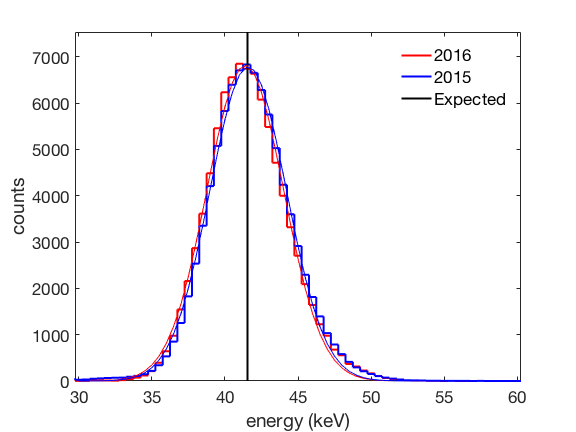
\includegraphics[width=6.5cm]{figures/KrEnergy.png} }}
\qquad
\subfloat{{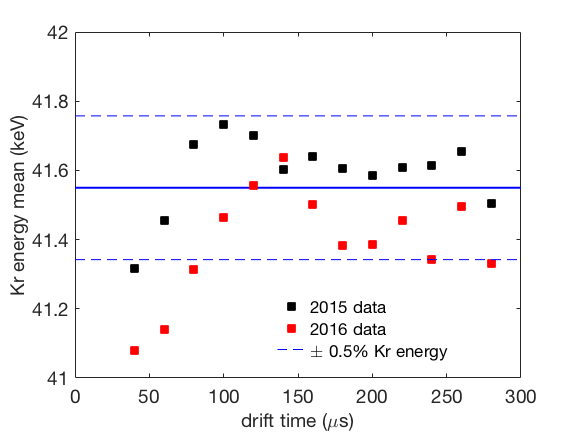
\includegraphics[width=6.5cm]{figures/KrEnergyZDep.png} }}
\caption{ (Left) The energy spectrum of $^{83m}$Kr data in September 2014 (red) and September 2015(blue) after determining the S1 field effect to S1a/S1b relationship from the reduced $\chi^2$ method. The energy spectrum is expected to be a Gaussian distribution centered around the black line.  (Right) The Z dependence of the $^{83m}$Kr energy peaks in September 2014 (red) and September 2015 (black).}
\label{Kr2p22_KrE}
\end{figure}

The CH$_3$T energy spectra from calibrations in September 2014, November 2014, February 2015, September 2015, and February 2016 are shown in figure \ref{Kr2p22_H3E}.  The fractional difference between the expected CH$_3$T spectrum and the CH$_3$T is shown below each energy spectrum.  Fractional residuals of up to 3 $\sigma$ are comparable to our CH$_3$T results from Run03.


\begin{figure}
%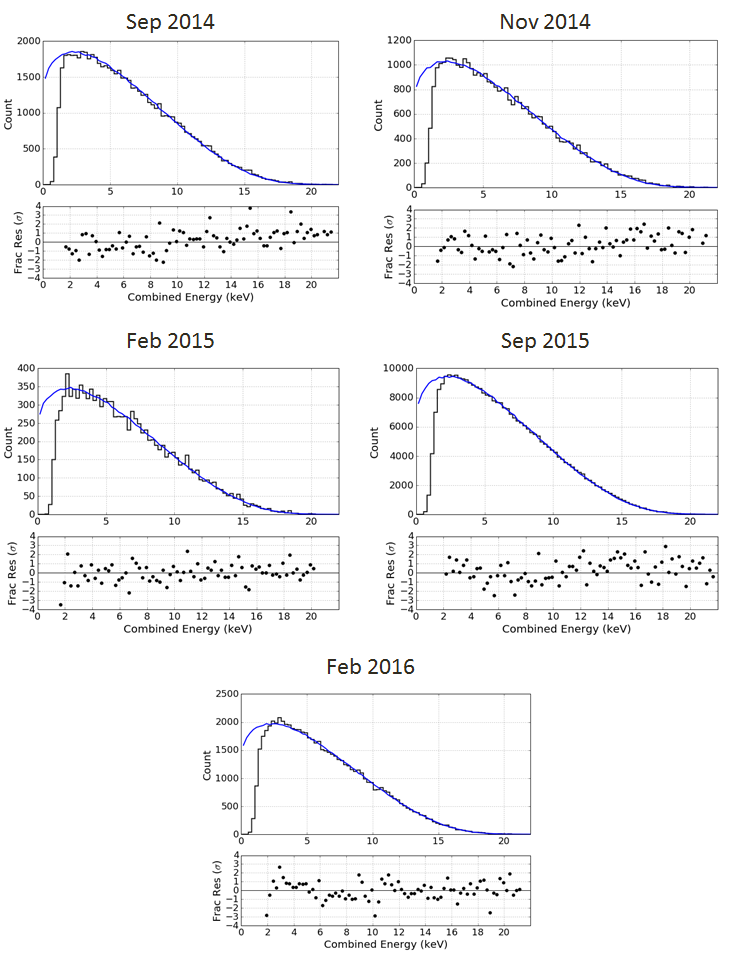
\includegraphics[scale=0.4]{figures/KrypCal_2p22_AllCH3TEnergy.png}
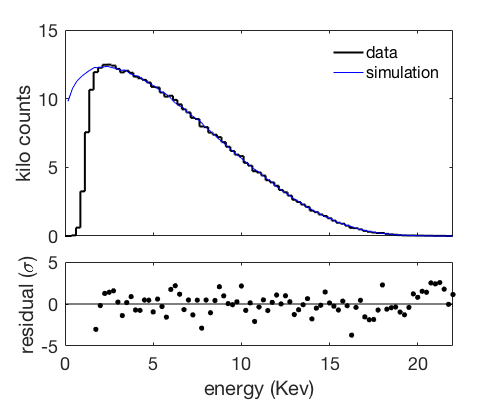
\includegraphics[scale=0.4]{figures/CH3T_energy_wres_sep2015.png}
\captionof{figure}{The September 2015 CH$_3$T energy spectra resulting from KrypCal corrections.}
 \label{Kr2p22_H3E}
\end{figure}


A version of the corrections which do not acknowledge the spatial and time dependent field in WS2014-16 returns best fit values of $g_1=0.100 \pm 0.001$ and extraction efficiency of EE$=1.08 \pm 0.030$.  This optimal value of the extraction efficiency is 40\%-80\% higher than our expectations based on Guschin data and our extraction field strength, and exceeds 100\% (Figure \ref{EEexpec}).  The $^{83m}$Kr and CH$_3$T energy spectra also produce an worse average reduced $\chi^2$ of 1.12 for the $^{83m}$Kr and CH$_3$T energy spectra when compared to the expected energy spectra, with a reduced $\chi^2$ of 10.06/26=0.3869 for $^{83m}$Kr alone, and a reduced $\chi^2$ of 230.2/124=1.8562 for CH$_3$T alone. 

\subsection{G1 and EE}

The $\chi^2$ method presented in section \ref{section:S1relation2} finds best fit values of $g_1=0.098 \pm 0.001$ and $EE=0.808 \pm 0.029$.  This is consistent with our expectations of an extraction efficiency between 0.6 and 0.8, based on our extraction field models and the liquid level, and is much better than the $g_1=0.100 \pm 0.001$ and $EE=1.08 \pm 0.030$ result found in section \ref{Result:Spectra}.  Likewise, the best fit value of $g_1$ is within one sigma of our expectation of g$_1$=0.108 $\pm$ 0.010 found in section \ref{G1pred}. 

\begin{center}
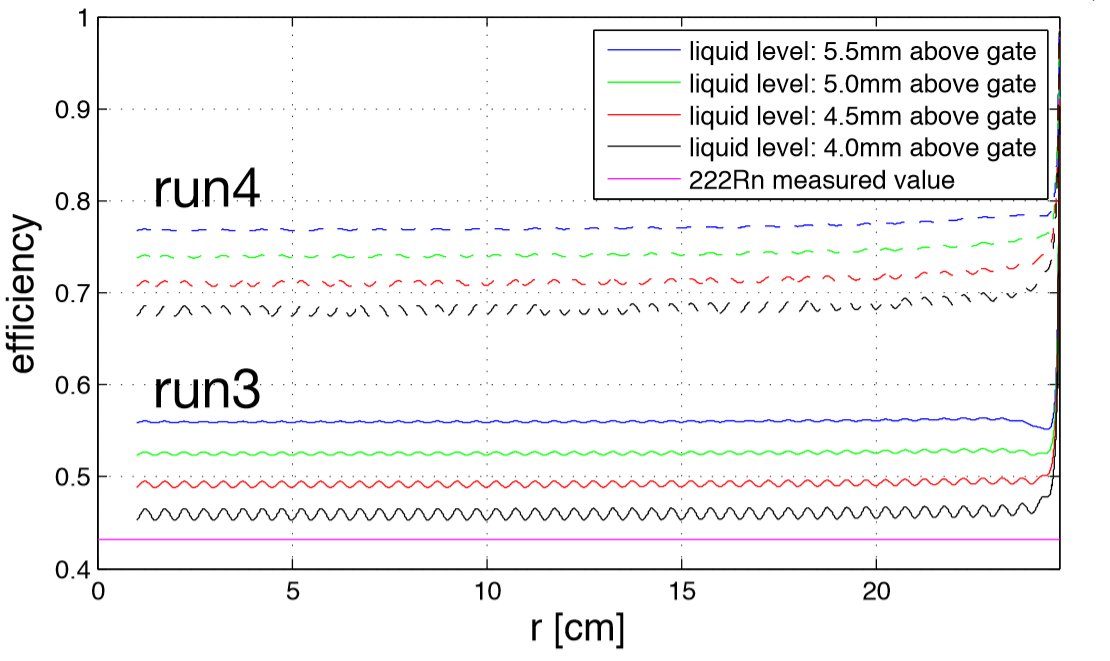
\includegraphics[scale=0.3]{figures/GuschinEE.png}
\captionof{figure}{The expected extraction efficiency based on the electric field map.  The expectation is derived from a Guschin curve, and is dependent on the height of the liquid above the gate.  The exact liquid level is unknown, so a range of possible values is depicted.}
 \label{EEexpec}
\end{center}


\subsection{Lifetime Estimates}

The nonuniform field in the LUX detector produces higher recombination of $^{83m}$Kr events in the bottom of the detector.  This results in an attenuation of the $^{83m}$Kr S2 signal that is directly proportional to drift time.  This effect mimics the attenuation of the $^{83m}$Kr S2 signal produced by impurities capturing charge as it drift to the top of the detector.  As a result, when field effects are not properly accounted for in a $^{83m}$Kr calibration, the electron lifetime is drastically underestimated.  The version of the corrections which does not account for field effects in WS2014-16 measured electron lifetimes below 350 $\mu$seconds at all points in time.  This problem is rectified by the methods presented here, which measure accurately measure the electron lifetime to be as high as a few milliseconds (Figure~\ref{fig:KrypCalLifetime}). The higher values of electron lifetimes have been confirmed by a separate, low energy $^{37}$Ar injection performed at the end of LUX's WS2014-16 data collection.

\begin{center}
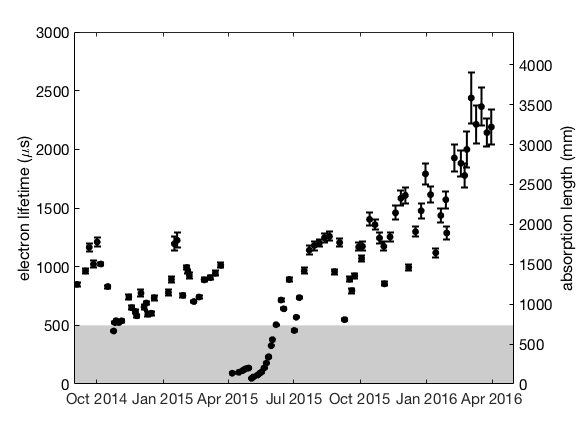
\includegraphics[scale=0.4]{figures/LUX_eLifetime_Kr2p22.png}
\captionof{figure}{The electron lifetime over WS2014-16 found by fitting an exponential to the S2$_F$ Z dependence.  Red areas indicate circulation outages.  At high lifetimes the S2$_F$ Z dependence is less exponential, leading to larger errors on the measurement.}
 \label{fig:KrypCalLifetime}
\end{center}

\subsection{Nuclear Recoil Band}

Nuclear recoils are much less sensitive to field variation effects in the detector, so a significant spatial dependence in the NR band it would indicate a flaw in the corrections. With the methods presented here, LUX's multi-Z NR band calibration in October 2014 shows $\sim4\%$ spatial dependence in the NR band, which is consistent with expectations from NEST (Figure \ref{NRBandZ}) . The result of the same calibration using a version of the corrections which do not properly account for field effects is also shown in Figure \ref{NRBandZ}.  The underestimate of the electron lifetime and subsequent over correction of the S2 data produces a large, non-physical z dependence in the NR band when field effects are not accounted for.  

\begin{figure}
\centering
\subfloat{{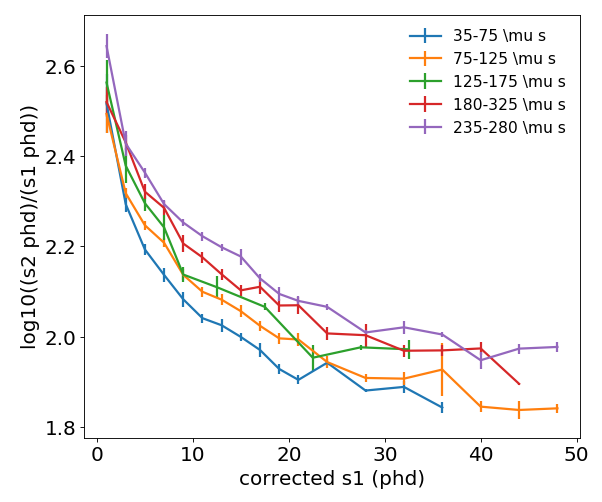
\includegraphics[width=6.5cm]{figures/NRband_run3.png} }}
\qquad
\subfloat{{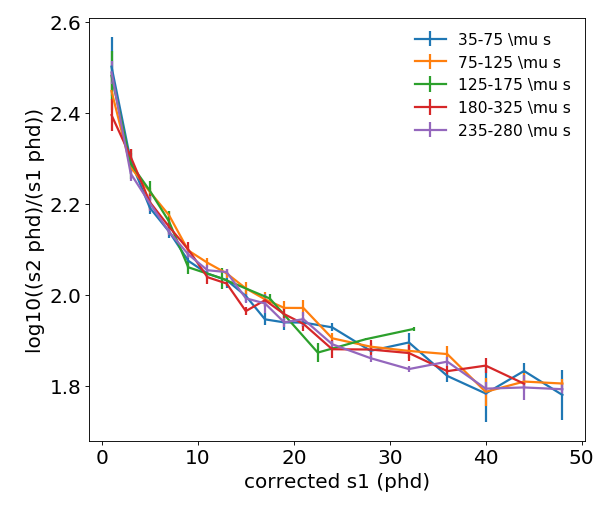
\includegraphics[width=6.5cm]{figures/NRband_run4.png} }}
\caption{ (Top) The Z dependence of the NR band mean using a version of KrypCal which does not properly account for field effects. (Bottom) The Z dependence of the NR band mean from the same datasets using a version of KrypCal which does properly account for field effects.  }
\label{NRBandZ}
\end{figure}

\subsection{Electron Recoil Band}

The electron recoil band that results from the corrections which do account for field effects should have significant spatial and time dependence due to the recombination variation induced by the nonuniform electric field remaining in the data. The corrected ER band calibration data from September 2015 was divided into three dimensional voxels with a height of 86 $\mu$seconds and an X and Y width of 16 cm.  We see a 16\% spatial variation of the ER band in September 2015 (at S1=20 phd), which is comparable to the libNEST prediction of a 13\% spatial variation (at S1=20 phd).  We also observe a $\sim$1\% variation in time for the total ER band over the duration of WS2014-16 (Figure \ref{ERBandVariation}). The relative size of the spatial and time dependence of the ER band is consistent with expectations, since the spatial dependence of the electric field is stronger than the time dependence of the electric field. 

%The spatial variation quoted is measured at S1c=20 phd

\begin{figure} 
\centering
\subfloat{{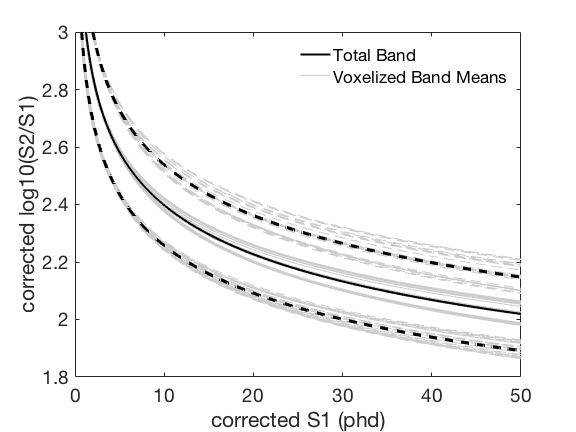
\includegraphics[width=6.5cm]{figures/Sep2015_VoxelizedBands_WithUpperLower.png} }}
\qquad
\subfloat{{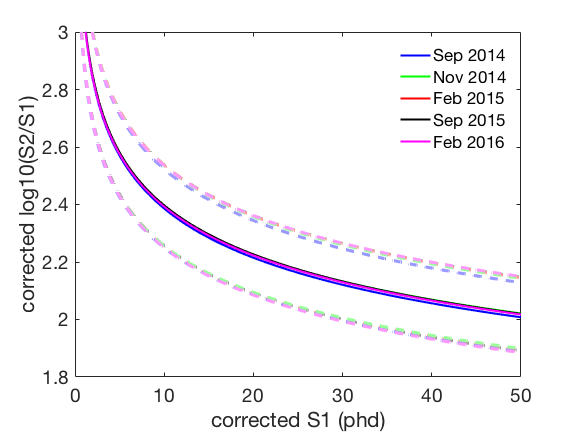
\includegraphics[width=6.5cm]{figures/OverlayOfAllERBands.png} }}
\caption{ (Left) The spatial variation of the KrypCal corrected ER band from September 2015.  The black band represents the total, unbinned ER band and the grey bands represent the ER band from each voxel. (Right) The time dependence of the total, unbinned ER band as measured by the KrypCal corrected data at four points in time.}
\label{ERBandVariation}
\end{figure}

Further evidence that the corrections are behaving properly appears in the ER band's electric field dependence.  We fit a power low to the ER band in September 2015 and relate the fit parameters to the S1a/S1b ratio.  We observe the polynomial relationships shown in Figure~\ref{ERBand_S1aS1bToER}.  These measured relationships can be used to reconstruct the ER band from any of the seven tritium calibrations that were acquired during Run04, from measurements of S1a/S1b alone.  Each of the reconstructed bands are within 3\% of the measured the ER bands, with p-values close to 1 in all cases.  

Figure~\ref{Feb2016ERPred} shows the close agreement between the ER band predicted from the polynomial relationships shown in Figure~\ref{ERBand_S1aS1bToER} to the ER band measured in data.  The predicted ER band was produced prior to measurement of the ER band in data.  Although not shown, the spatial dependence of the ER band is also reproduced within 2\% of the measured band. 

\begin{figure} 
\centering
\subfloat{{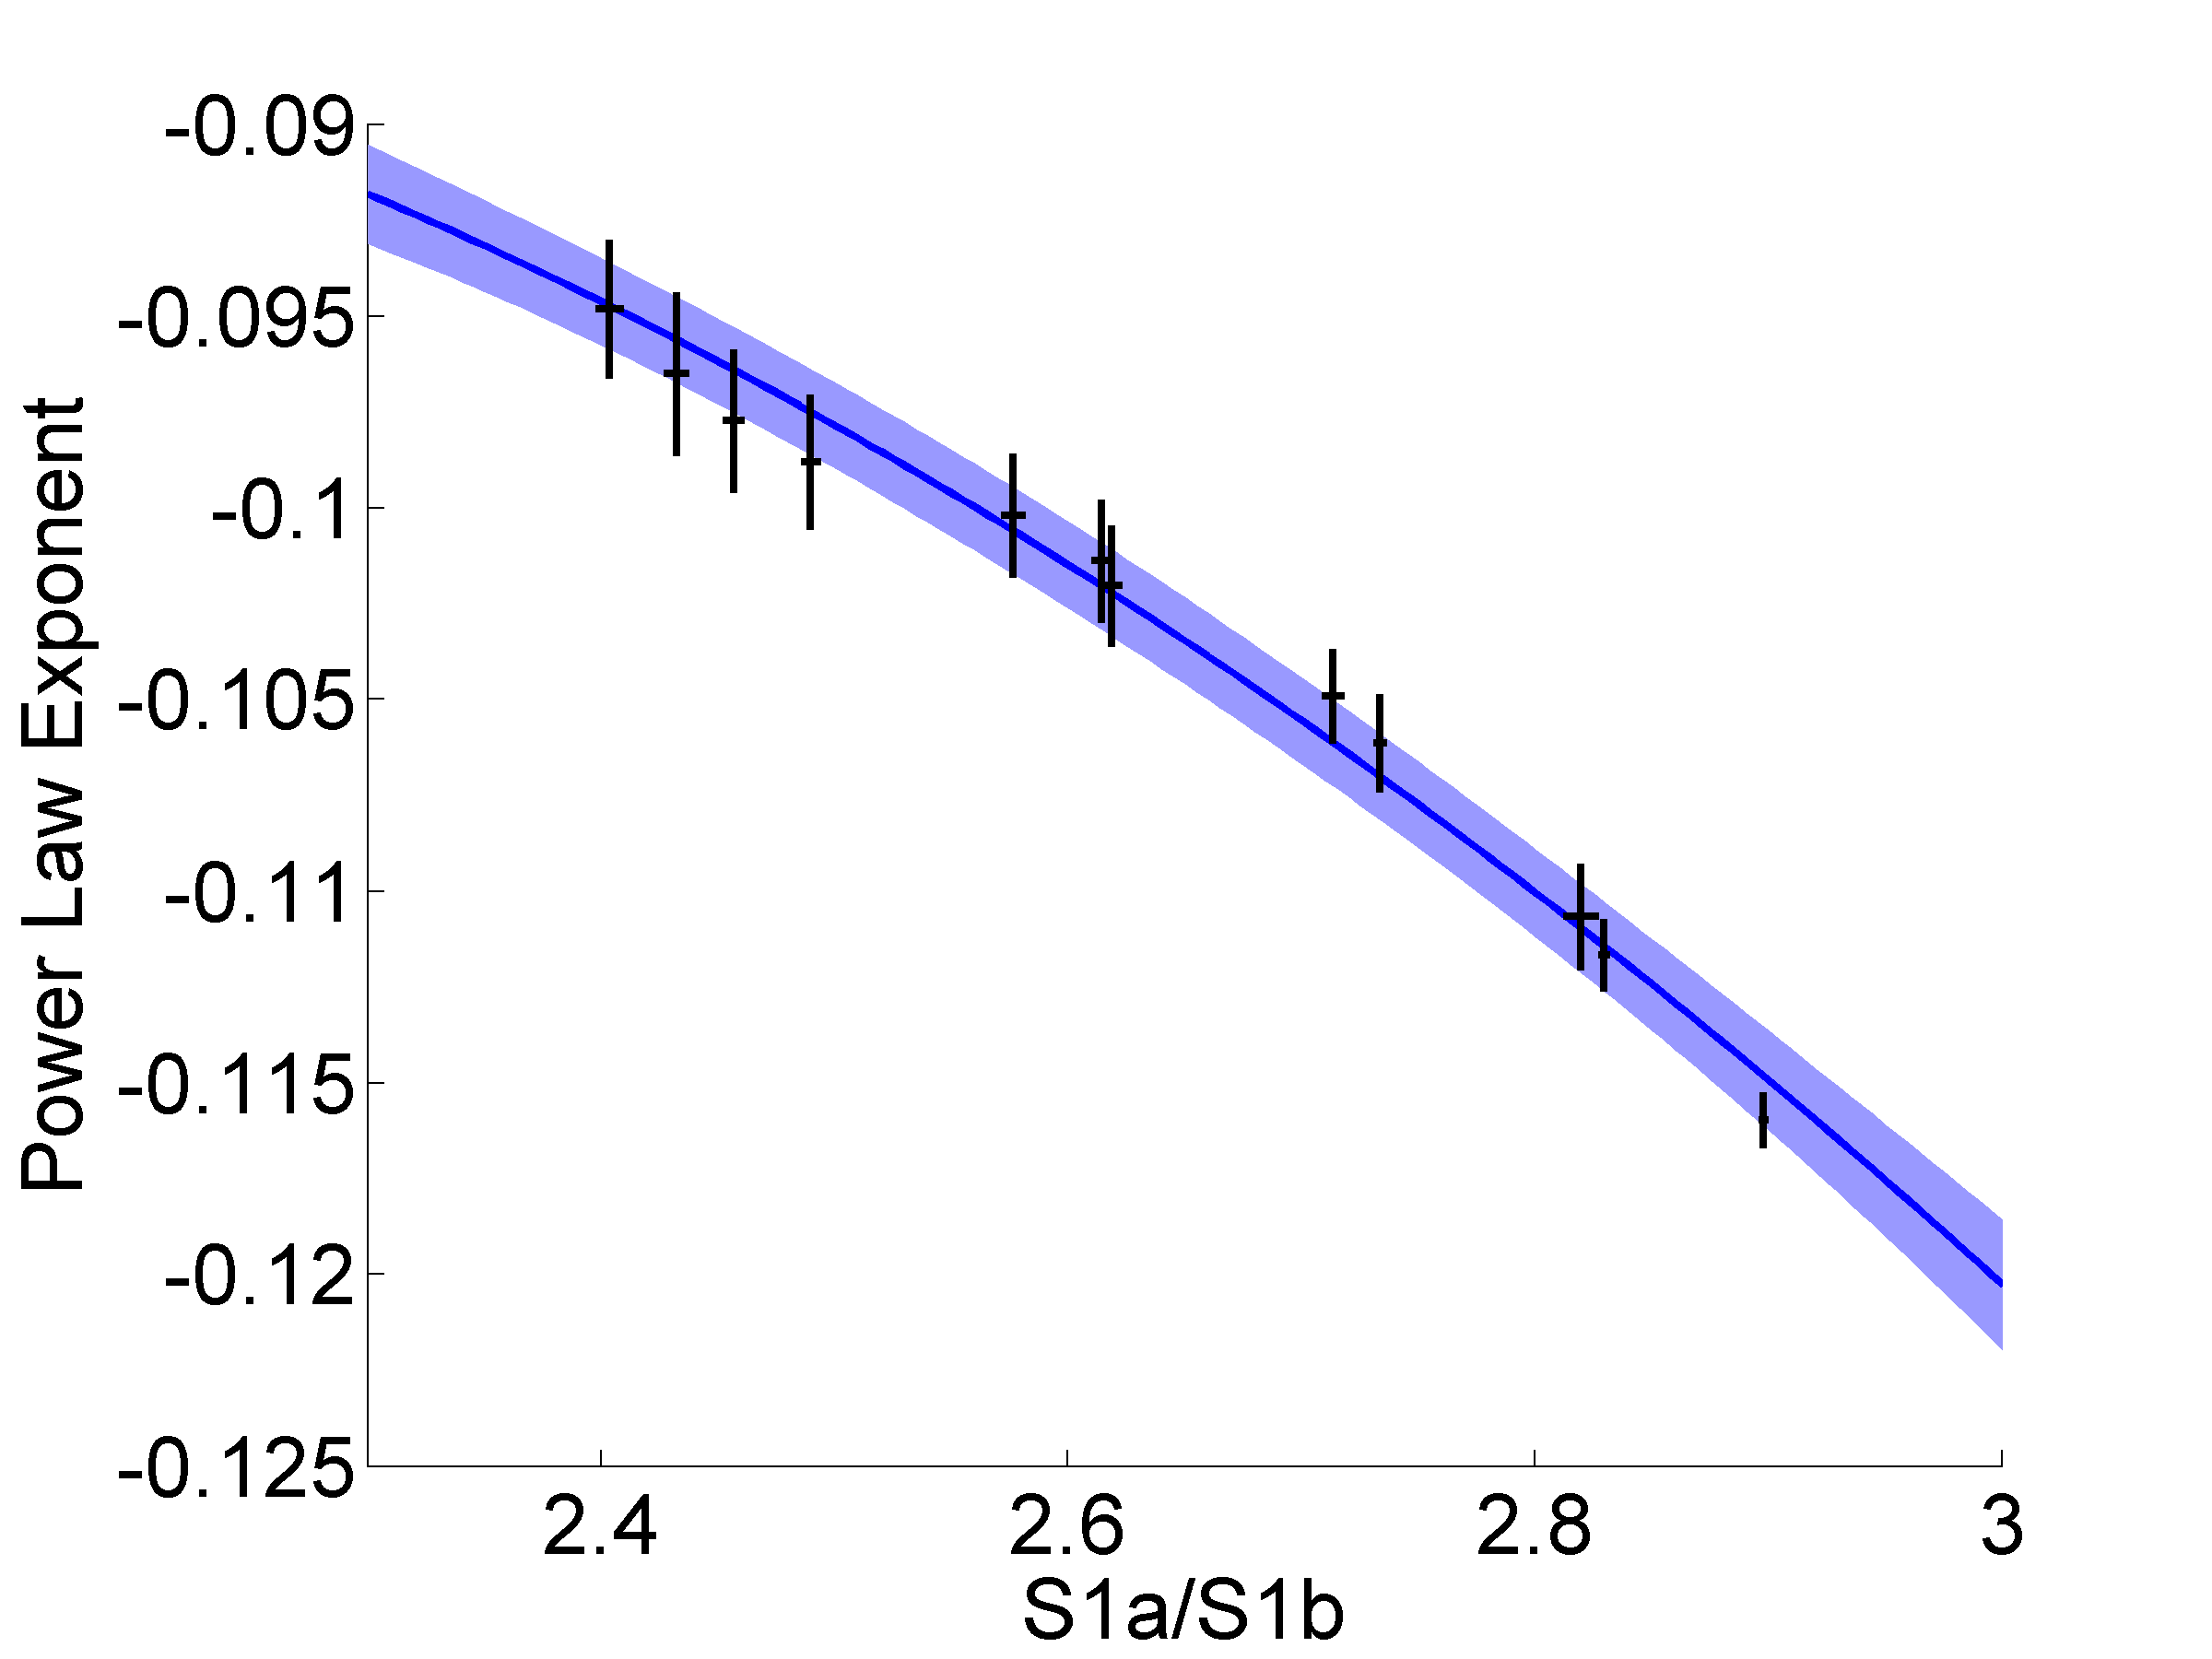
\includegraphics[width=6.5cm]{figures/PowerLawExponent.png} }}
\qquad
\subfloat{{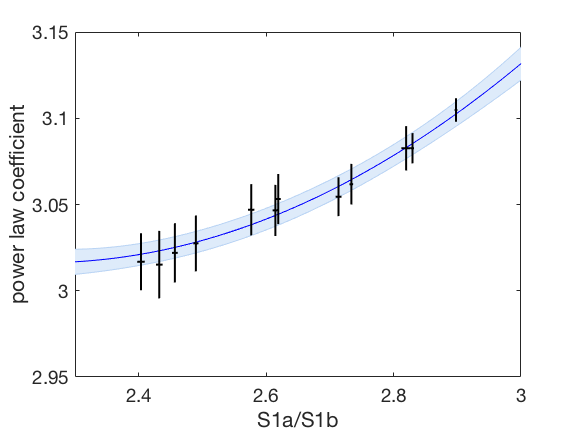
\includegraphics[width=6.5cm]{figures/PowerLawCoefficient.png} }}
\caption{ (Left) The measured relationship between S1a/S1b and the ER band power law exponent. (Right) The measured relationship between S1a/S1b and the ER band power law coefficient. The light blue region indicates one $\sigma$ uncertainties on each fit.}
\label{ERBand_S1aS1bToER}
\end{figure}


\begin{center}
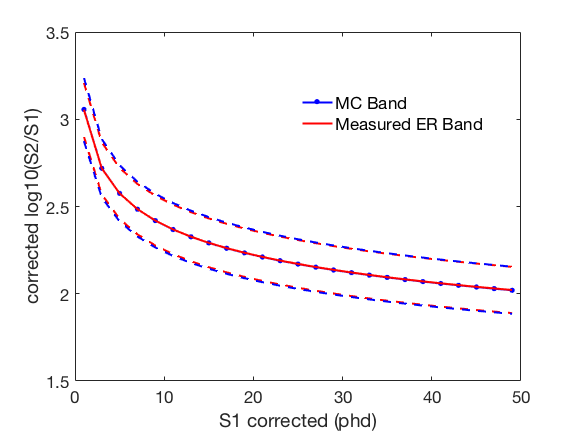
\includegraphics[scale=0.45]{figures/Feb2016_ERPrediction.png}
\captionof{figure}{Monte Carlo data for the February 2016 ER band generated from S1a/S1b using the relationship found in Figure \ref{ERBand_S1aS1bToER}.  A fit to the Monte Carlo data is shown in blue, and a fit to the actual calibration data (not shown) is shown in red.}
 \label{Feb2016ERPred}
\end{center}



\section{Conclusions}

LUX's WS2014-16 data is complicated by a nonuniform electric field in the detector.  The variation of the electric field in space and time produces variation in the recombination of S1 and S2 events as a function of energy, time, space, and recoil type.  If this recombination variation is not properly separated from detector inefficiency effects in $^{83m}$Kr data, the KrypCal corrections produce data which has poor energy reconstruction with unreasonably high extraction efficiency estimates, worsened energy resolution, and widened ER bands.  We have developed multiple methods to relate the strength of the field effect in S1 and S2 data to the $^{83m}$Kr S1a/S1b ratio.  These two relationships can be used to separate the field effects from detector inefficiency effects prior to producing KrypCal corrections from $^{83m}$Kr calibrations taken at any point in time.  This process results in better energy reconstruction with g1 and extraction efficiency values close to our expectations,  improved energy resolution, and improved ER band width.  However, since the field effects remain in the corrected data, a spatial and time dependence remain in the corrected S1 and S2 signal, leading to complications in calibrating the corrected ER band over time.



\appendix

%\section{Studies of the removal of CH$_3$T from LXe }
\label{sec:appendix1}

\newcommand*{\Scale}[2][4]{\scalebox{#1}{$#2$}}%

Prior to the first injection of CH$_3$T into LUX, we considered three risks that such a calibration may pose to the dark matter search: 1) that the xenon purification system may be ineffective for CH$_3$T removal; 2) that the interior surfaces of the stainless steel (SS)  gas handling system may become permanently contaminated with CH$_3$T; and 3) that the plastic detector components may outgas unacceptable quantities of CH$_3$T after initial exposure.

To address the first concern we studied the removal of natural methane (CH$_4$) from Xe gas with a heated Zr getter and a mass spectrometer. The purification efficiency was found to be satisfactory~\cite{Dobi_CH4}. Furthermore, a test of the completed LUX purification system, including the actual getter unit, was performed several weeks before the first CH$_3$T injection into LUX. In this test $\sim$0.1 grams of CH$_4$ was injected into LUX, and mass spectrometry measurements of the CH$_4$ concentration in the LUX Xe gas were performed over the next several days. The CH$_4$ concentration was observed to decrease exponentially with a time constant of 5.90 $\pm 0.07$ hours as shown in Fig.~\ref{fig:ch4_removal}, confirming the effectiveness of the purification system for methane removal.

The behavior of CH$_3$T in SS plumbing was studied in a bench-test with a custom-built Xe gas proportional tube operated at room temperature. Substantial quantities of CH$_3$T activity were injected, counted, and removed from the proportional tube. Initial tests found a small amount of residual activity after purification, however this was resolved by passing the CH$_3$T through a methane purifier (SAES model MC1-905F). No subsequent contamination was observed.

\begin{figure}[h!]
\includegraphics[width=80mm]{fig14.pdf}
\caption{Injection and removal of CH$_4$ in LUX prior to the first CH$_3$T injection. CH$_4$ is observed with a gas sampling mass spectrometry system. The black dashed lines shows an exponential fit to the CH$_4$ concentration at the detector return line with a time constant of 5.90 $\pm 0.07$ hours.  The red points indicate measurements at the getter outlet. We find a 97\% one-pass removal efficiency at a flow rate of 27 slpm. The blue curve shows the upper limit on the effect of outgassing from the plastics. The three data points near t = 3 days are consistent with the limit of detection for methane ($\sim \rm 5\times10^{-3}$ ppb (g/g)) .}
\label{fig:ch4_removal}
\end{figure}

We also performed tests of CH$_3$T injection and removal from LXe with a small detector. One such experiment is shown in Fig.~\ref{fig:Density}, where 68,000 Hz of CH$_3$T was injected, counted, and subsequently removed from LXe. Samples of LUX polyethylene and teflon were immersed in the LXe in this experiment, and their outgassing is evident in Fig.~\ref{fig:Density}. These data placed constraints on the risk of CH$_3$T outgassing in LUX. In total over one million Hz of CH$_3$T activity was injected and successfully removed in these experiments. 

\begin{figure}[h!]
\includegraphics[width=80mm]{fig15.pdf}
\caption{The event rate versus time following a large CH$_3$T injection into a bench-top liquid xenon detector. Black points: the event rate measured with a dead-time limited digital DAQ system. Grey points: true event rate measured with a fast analog scalar. In this experiment a maximum activity of 68,000 Hz was detected immediately after the injection, compared to a background count rate of 5 Hz. Initially the purifier is not included in the recirculation circuit, leading to a constant count rate. The count rate falls rapidly when the purifier is activated. At 0.5 days an elbow in the count rate is observed, indicating that outgassing of CH$_3$T from the detector plastics has become a limiting factor in the purification rate. }
\label{fig:Density}
\end{figure}

As a final measure of risk mitigation, the CH$_3$T injection into LUX was performed at the end of Run 3 after the WIMP search data had been collected.

\section{Model of CH$_3$T removal}
\label{sec:appendix2}

We use a simple purification model to predict the CH$_3$T activity in LUX after an injection. The model is 

\begin{equation}
\frac{dC}{dt} = \frac{A}{V}J_{out} -\frac{C}{\tau},
\end{equation}

\noindent where  $C$ is the CH$_3$T concentration in the LXe,  $J_{out}$ is the flux of CH$_3$T out of the plastic components due to outgassing,  $A$ is the surface area of the plastic TPC cylinder, $V$ is the total volume of xenon in the active region, and $\tau$ is the characteristic removal time of CH$_3$T due to purification (5.9 hours). The model assumes perfect mixing of the fluid in the TPC, similar to what has been observed in LUX. The initial concentration is the injection activity divided by the volume of the active region. We solve the model numerically with the Euler method while simultaneously solving the diffusion equation to determine $J_{out}$. The results predict the number of calibration events that may be collected and provide an estimate of when the CH$_3$T  decay rate will be small enough to allow the WIMP search to resume.

We approximate the diffusion into and out of the plastics as one-dimensional, since most plastics in LUX can be approximated as a thin cylindrical shell with no dependence on the azimuthal or $z$ coordinates.  Fick's laws in one dimension are

\begin{align}
J=-D\frac{d \phi(r,t)}{d r}  \\
\frac{d \phi}{d t} = D \frac{d^2 \phi(r,t)}{d r^2} , 
\end{align}

\noindent 
where $J$ is the flux, $\phi(r,t)$ is the CH$_3$T  concentration in the plastic at depth $r$ and time $t$, and $D$ is the diffusion constant in the plastic. The concentration at the LXe-plastic boundary is fixed at $KC$, where K is the unitless solubility of CH$_3$T in the plastics. These equations are solved numerically and simultaneously with the purification model. 

$D$ and $K$ are not independently known for CH$_3$T in teflon or polyethylene at LXe temperature. However, only the combined quantity $G \equiv K \sqrt{ D/ \pi }$ is relevant as long as the diffusing substance does not reach the center of the plastic component (a good assumption for diffusion of CH$_3$T at LXe temperature). Under this condition, there exists an analytic solution to Fick's first law, which we evaluate at the LXe boundary:

%\begin{equation}
%\Scale[0.75]{\phi (x,t) = KC - \int \limits_0^t erf(\frac{x}{\sqrt{4D(t - \tau)}})K\frac{d}{d\tau}C(\tau)d\tau - KC(0)erf(\frac{x}{\sqrt{4Dt}}),}
%\end{equation}

\begin{equation}
J_{out}(t)= - G\left( \int \limits_0^t \frac{\frac{d}{dt'}C(t')}{\sqrt{t-t'}} dt' + \frac{C(0)}{\sqrt{t}}\right),
\end{equation}

\noindent
where the sign is reversed because the flux of material is outward. This result can be derived by applying Duhamel's principle along the infinite half-line, and it shows that the outgassing flux is linear in $G$. We set an upper limit of $G<0.0016 \frac{cm}{\sqrt{day}}$ for LUX based upon the data in Fig.~\ref{fig:ch4_removal}. In that data the effect of $G$ would appear as an elbow in the CH$_4$ concentration versus time, as indicated by the blue line. The three data points near t = 3 days constrain the maximum value of $G$. We interpret this result as an upper limit because those data points are consistent with CH$_4$ backgrounds in the mass spectrometry system.

\begin{figure}[h!]
\includegraphics[width=0.95\textwidth]{fig16.pdf}
\caption{Results of the purification model from 1 Bq (black curve) and 10 Bq (red curve) injections of CH$_3$T into LUX. The dashed blue line is the tritium activity goal of 0.33 $\mu$ Bq. The sharp initial fall is due to the 5.9 hour purification time constant of LUX, while the slow long-term removal is dominated by outgassing. The outgassing simulated here assumes  $G=0.0016$ cm/day$^{1/2}$).}
\label{fig:tau_var}
\end{figure}

Fig.~\ref{fig:tau_var} shows the results of the purification model for a 1 Bq and 10 Bq injection into LUX assuming $G$ = 0.0016 cm/day$^{1/2}$  . We take 0.33 $\mu$Bq of residual CH$_3$T activity as an approximate goal for resuming WIMP search running, and we find that for injections on the order of 1 Bq we reach 0.33 $\mu$Bq eight days later, while 10 Bq injections may take as long as 35 days.  Ultimately the final decision regarding low background data quality is made during the data analysis phase, with guidance provided by the purification model described here.


\section{Light and charge yields of electron recoils in LXe at 180~V/cm and 105~V/cm}
\label{sec:appendix3}

Tables~\ref{table:Yields} and \ref{table:Yields_100} list the light and charge yields of LXe for ER events between 1.3 and 17 keV and at fields of 180~V/cm and 105~V/cm, respectively. The uncertainties on the light and charge yields are highly anti-correlated in each energy bin due to the way in which the gain factors $g_1$ and $g_2$ are measured. The uncertainty listed includes both statistical and the dominant systematic uncertainty from the constraint on $g_1$ and $g_2$.

\begin{table}[h!]
\centering
\begin{tabular}{|c|c|c|c|} \hline
Energy 	& 		LY	& 	QY	& $\sigma$ \\ 
$\rm (keV_{ee}$) & ($\rm n_\gamma$/keV)   & ($\rm n_e$/keV) & ($\rm n$/keV) \\ \hline
1.3 	 & 14.6 	 & 58.4 	 & 2.2 	 \\ \hline 
1.5 	 & 17.3 	 & 55.7 	 & 1.9 	 \\ \hline 
2.0 	 & 22.3 	 & 50.7 	 & 2.4 	 \\ \hline 
2.5 	 & 27.4 	 & 45.6 	 & 2.5 	 \\ \hline 
3.0 	 & 31.5 	 & 41.4 	 & 2.3 	 \\ \hline 
3.5 	 & 33.8 	 & 39.2 	 & 2.0 	 \\ \hline 
4.0 	 & 35.8 	 & 37.2 	 & 2.2 	 \\ \hline 
4.5 	 & 37.5 	 & 35.5 	 & 2.0 	 \\ \hline 
5.0 	 & 38.4 	 & 34.6 	 & 1.9 	 \\ \hline 
5.2 	 & 38.9 	 & 34.1 	 & 2.0 	 \\ \hline 
5.5 	 & 39.5 	 & 33.5 	 & 2.1 	 \\ \hline 
6.0 	 & 40.4 	 & 32.6 	 & 2.0 	 \\ \hline 
6.5 	 & 41.7 	 & 31.3 	 & 2.0 	 \\ \hline 
7.0 	 & 41.7 	 & 31.3 	 & 1.7 	 \\ \hline 
7.5 	 & 42.7 	 & 30.3 	 & 2.0 	 \\ \hline 
8.0 	 & 42.9 	 & 30.1 	 & 1.9 	 \\ \hline 
9.0 	 & 43.8 	 & 29.1 	 & 1.7 	 \\ \hline 
10.0 	 & 44.7 	 & 28.3 	 & 2.0 	 \\ \hline 
11.0 	 & 45.4 	 & 27.6 	 & 1.7 	 \\ \hline 
12.0 	 & 46.0 	 & 27.0 	 & 1.7 	 \\ \hline 
13.0 	 & 46.5 	 & 26.5 	 & 1.5 	 \\ \hline 
14.0 	 & 47.1 	 & 25.9 	 & 1.6 	 \\ \hline 
16.0 	 & 46.4 	 & 26.6 	 & 2.5 	 \\ \hline 
17.0 	 & 44.9 	 & 28.1 	 & 2.5 	 \\ \hline 
\end{tabular}
\caption{Light and charge yield (photons/keV and electrons/keV) measured with tritium decay at 180~V/cm. The uncertainty includes both statistical and the dominant systematic uncertainty, common for both, from the constraint on $g_1$ and $g_2$.}
\label{table:Yields}
\end{table}

\begin{table}[h!]
\centering
\caption{Light and charge yield (photons/keV and electrons/keV) measured with tritium decay at 105~V/cm. The uncertainty includes both statistical and the dominant systematic uncertainty, common for both, from the constraint on $g_1$ and $g_2$. The available statistics in this data is smaller than that of the 180~V/cm data , resulting in fewer energy bins.}
\begin{tabular}{|c|c|c|c|} \hline
Energy 	& 		LY	& 	QY	& $\sigma$ \\ 
$\rm (keV_{ee}$) & ($\rm n_\gamma$/keV)   & ($\rm n_e$/keV) & ($\rm n$/keV) \\ \hline
1.3 	 & 18.4 	 & 54.6 	 & 1.7 	 \\ \hline 
2.2 	 & 25.1 	 & 47.8 	 & 1.9 	 \\ \hline 
3.1 	 & 33.4 	 & 39.6 	 & 2.2 	 \\ \hline 
4.0 	 & 37.6 	 & 35.4 	 & 2.3 	 \\ \hline 
4.9 	 & 39.9 	 & 33.1 	 & 1.7 	 \\ \hline 
5.8 	 & 41.3 	 & 31.6 	 & 2.2 	 \\ \hline 
6.7 	 & 43.0 	 & 29.9 	 & 2.0 	 \\ \hline 
7.6 	 & 44.1 	 & 28.9 	 & 1.6 	 \\ \hline 
8.5 	 & 46.2 	 & 26.8 	 & 2.0 	 \\ \hline 
9.4 	 & 46.2 	 & 26.8 	 & 2.0 	 \\ \hline 
10.3 	 & 47.7 	 & 25.3 	 & 1.5 	 \\ \hline 
11.2 	 & 46.8 	 & 26.2 	 & 1.5 	 \\ \hline 
12.1 	 & 49.1 	 & 23.9 	 & 1.9 	 \\ \hline 
13.0 	 & 49.6 	 & 23.4 	 & 1.5 	 \\ \hline 
13.9 	 & 50.8 	 & 22.2 	 & 3.2 	 \\ \hline 
15.0 	 & 49.2 	 & 23.7 	 & 1.4 	 \\ \hline 
16.4 	 & 46.3 	 & 26.7 	 & 2.2 	 \\ \hline 
\end{tabular}
\label{table:Yields_100}
\end{table}






\begin{acknowledgments}

This work was partially supported by the U.S. Department of Energy (DOE) under award numbers DE-FG02-08ER41549, DE-FG02-91ER40688, DE-FG02-95ER40917, DE-FG02-91ER40674, DE-NA0000979, DE-FG02-11ER41738, DE-SC0006605, DE-AC02-05CH11231, DE-AC52-07NA27344, and DE-FG01-91ER40618; the U.S. National Science Foundation under award numbers PHYS-0750671, PHY-0801536, PHY-1004661, PHY-1102470, PHY-1003660, PHY-1312561, PHY-1347449; the Research Corporation grant RA0350; the Center for Ultra-low Background Experiments in the Dakotas (CUBED); and the South Dakota School of Mines and Technology (SDSMT). LIP-Coimbra acknowledges funding from Funda\c{c}\~{a}o para a Ci\^{e}ncia e a Tecnologia (FCT)   through the project-grant PTDC/FIS-NUC/1525/2014. Imperial College and Brown University thank the UK Royal Society for travel funds under the International Exchange Scheme (IE120804). The UK groups acknowledge institutional support from Imperial College London, University College London and Edinburgh University, and from the Science \& Technology Facilities Council for PhD studentship ST/K502042/1 (AB). The University of Edinburgh is a charitable body, registered in Scotland, with registration number SC005336. This research was conducted using computational resources and services at the Center for Computation and Visualization, Brown University.

We gratefully acknowledge the logistical and technical support and the access to laboratory infrastructure provided to us by the Sanford Underground Research Facility (SURF) and its personnel at Lead, South Dakota. SURF was developed by the South Dakota Science and Technology Authority, with an important philanthropic donation from T. Denny Sanford, and is operated by Lawrence Berkeley National Laboratory for the Department of Energy, Office of High Energy Physics.

\end{acknowledgments}


%double blank page so that the table doesn't spill into the bibliography
\newpage
\thispagestyle{empty}
\mbox{}
\newpage
\thispagestyle{empty}
\mbox{}

%\input{Tritium.bbl}

\bibliography{KrypCal_Paper--KnocheDraft}

\end{document}